\documentclass[11pt,dvipdfmx,b5paper,oneside,report,uplatex]{jsbook}


\usepackage{color}
\usepackage{here}
\usepackage{framed}
\usepackage{tcolorbox}
\usepackage{quotchap}
\usepackage{pdfpages}
\usepackage[hidelinks]{hyperref}
\usepackage{pxjahyper}
\usepackage{titlesec}
\usepackage{picture}
\usepackage{tikz}
\usepackage{graphicx}
\usepackage{geometry}
\usepackage{url}
\usepackage{pdfpages}


\tcbuselibrary{breakable,listings}
\definecolor{shadecolor}{gray}{0.80}

% 余白を狭くする
\geometry{left=20mm,right=20mm,top=25mm,bottom=25mm}

% section
\titleformat{\section}[block]{}{}{0pt}
{
  \definecolor{teal}{gray}{0.30}
  \begin{picture}(0,0)
    \put(-10,-5){
      \begin{tikzpicture}
        \fill[teal] (0pt,0pt) rectangle (5pt,19pt);
      \end{tikzpicture}
    }
    \put(-10,-5){
      \color{teal}
      \line(1,0){\hsize}
    }
  \end{picture}
  \hspace{0pt}
  \sf \Large \thesection
  \hspace{0pt}
}

% 図表見出し
\renewcommand{\tablename}{\textcolor{gray}{▼} 表}
\renewcommand{\figurename}{\textcolor{gray}{▲} 図}

\begin{document}

\begin{titlepage}
  \newgeometry{left=0cm,right=0cm,top=0cm,bottom=0cm}
  \centering
  \includepdf[pages={1},width=\paperwidth,height=\paperheight]{./image/01-title/outside.pdf}
  \restoregeometry % 元の余白に戻す
\end{titlepage}
%目次を自動的に作る。
\tableofcontents
\chapter{初めに}

さて、みなさん。Webサイトは作られていますか?
Webサイトを作る時にそのままHTMLを触ってGithubなどで管理をしてもいいのですが、やはりGithubを使ったことない人にとってはWebサイトの更新だけでかなり大変な作業になってしまいます。

そこで、今サークルの情報共有で用いているesaを用いてWebサイトを更新したら簡単に、誰でも更新できるのではないかと考え、実装してみることにしました。
そこまで難しくないので、ぜひ参考にしてみてください。
\chapter{実際の動作しているサイト}

現在、下記レポジトリ、サイトで実際に動作しています。
実際にesaから記事を取り出して、Githubにpushしているので、記事を更新するだけで、Webサイトが更新されます。


レポジトリ:
\url{https://github.com/SystemEngineeringTeam/BlogSiteMarkDown}

Webサイト:
\url{https://esa.harutiro.net/}

\begin{figure}[htbp]
  \begin{minipage}{0.5\hsize}
      \begin{center}
          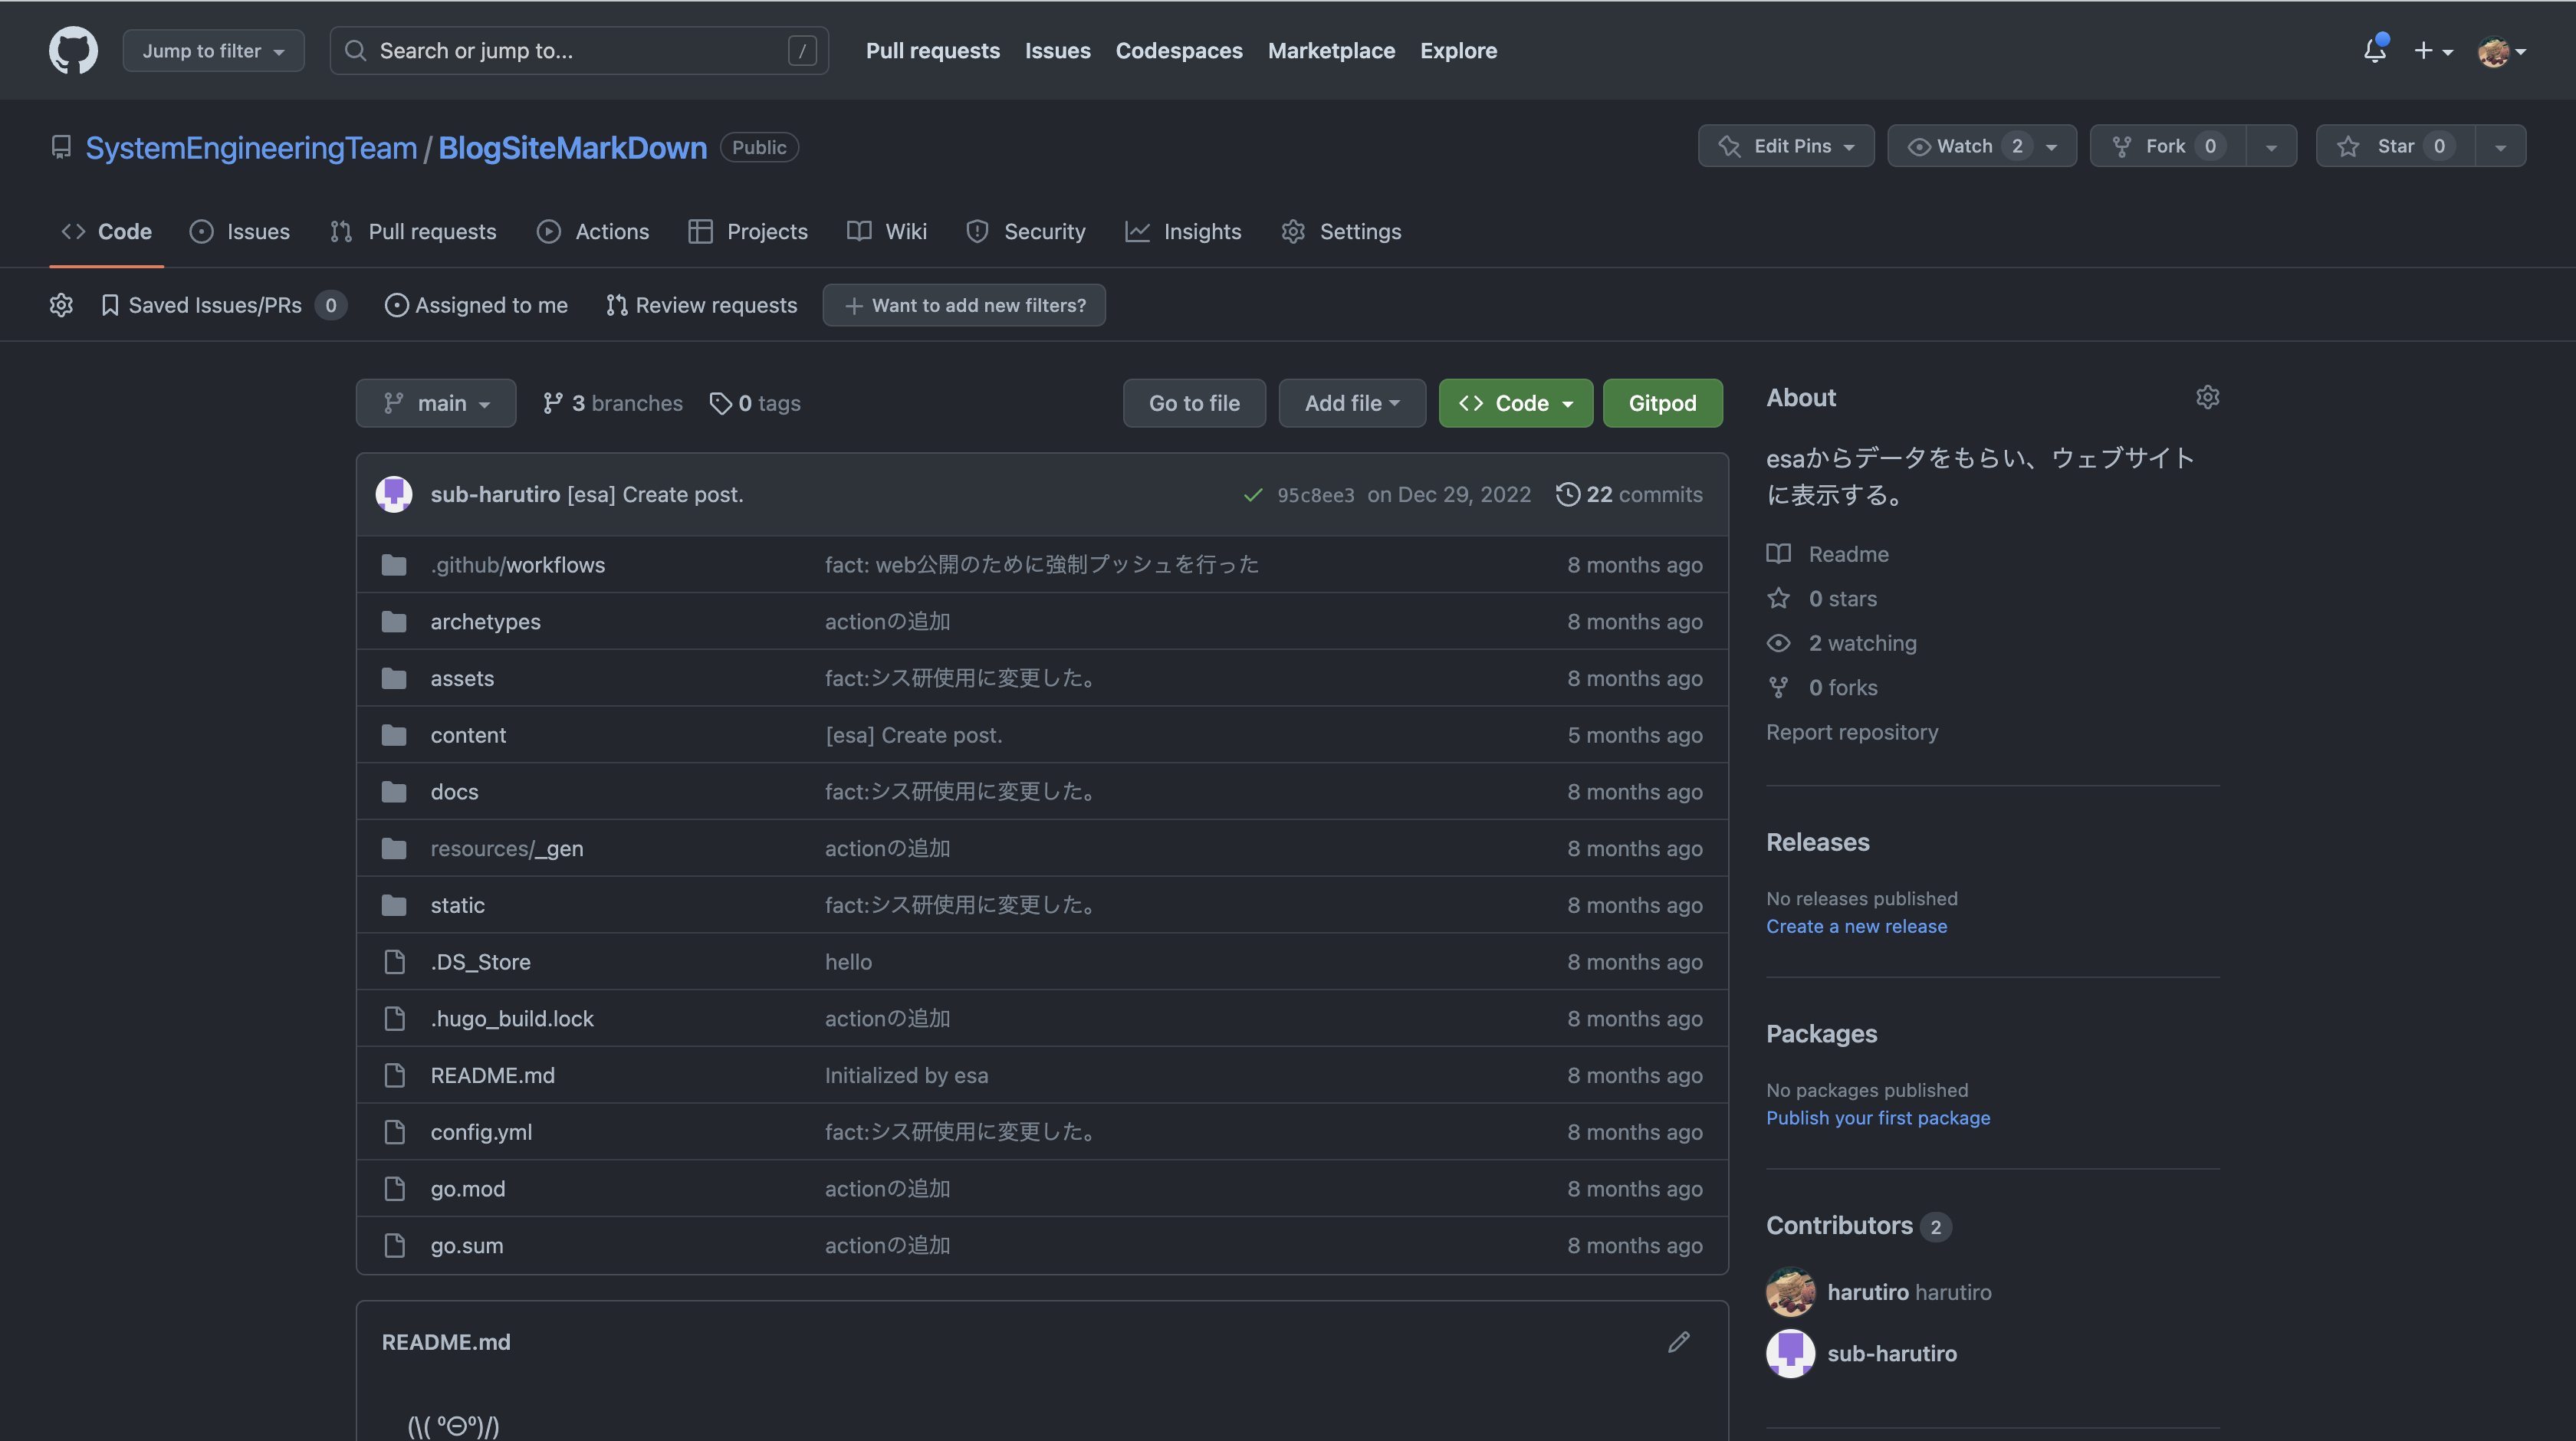
\includegraphics[width=50mm]{./image/02-chap2/git-repo.png}
      \end{center}
      \caption{Gitレポジトリ}
      \label{chap2-git-repo}
  \end{minipage}
  \begin{minipage}{0.5\hsize}
      \begin{center}
          
\includegraphics[width=50mm]{./image/02-chap2/sysken-web.png}
      \end{center}
      \caption{Webサイト}
      \label{chap2-web-site}
  \end{minipage}
\end{figure}
\chapter{用語まとめ}

\section{esa}

  \begin{figure}[H]
    \centering
    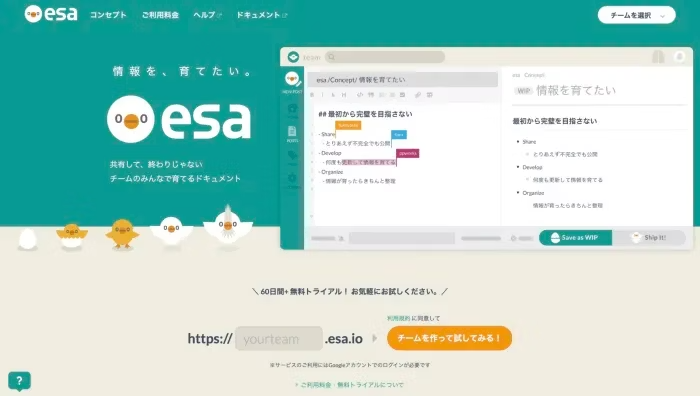
\includegraphics[width=6cm]{./image/02-chap3/esa.png}
    \caption{esaのホームページの写真}
    \label{chap3-esa-image}
  \end{figure}


  \begin{tcolorbox}[title=esaとは]
    esaとは、2014年に設立された合同会社esaの「情報共有ツール」です。
    esaは「不完全でも早い段階でチームに共有し、更新を重ねることでより良い情報に育つ」という発想のもと生まれました。そのため「Share(公開)」「Develop(更新して情報を育てる)」「Organize(育った情報を整理)」の3つの流れで設計されています。
    現在は3,000社を超える企業に導入されており、主に情報の蓄積やWIP機能(書いている途中でも共有する機能)を用いて、業務の効率化を実現している企業が多いです。
    \cite{esaとは} \cite{公式esaWeb}

  \end{tcolorbox}

\section{hugo}

  \begin{figure}[H]
    \centering
    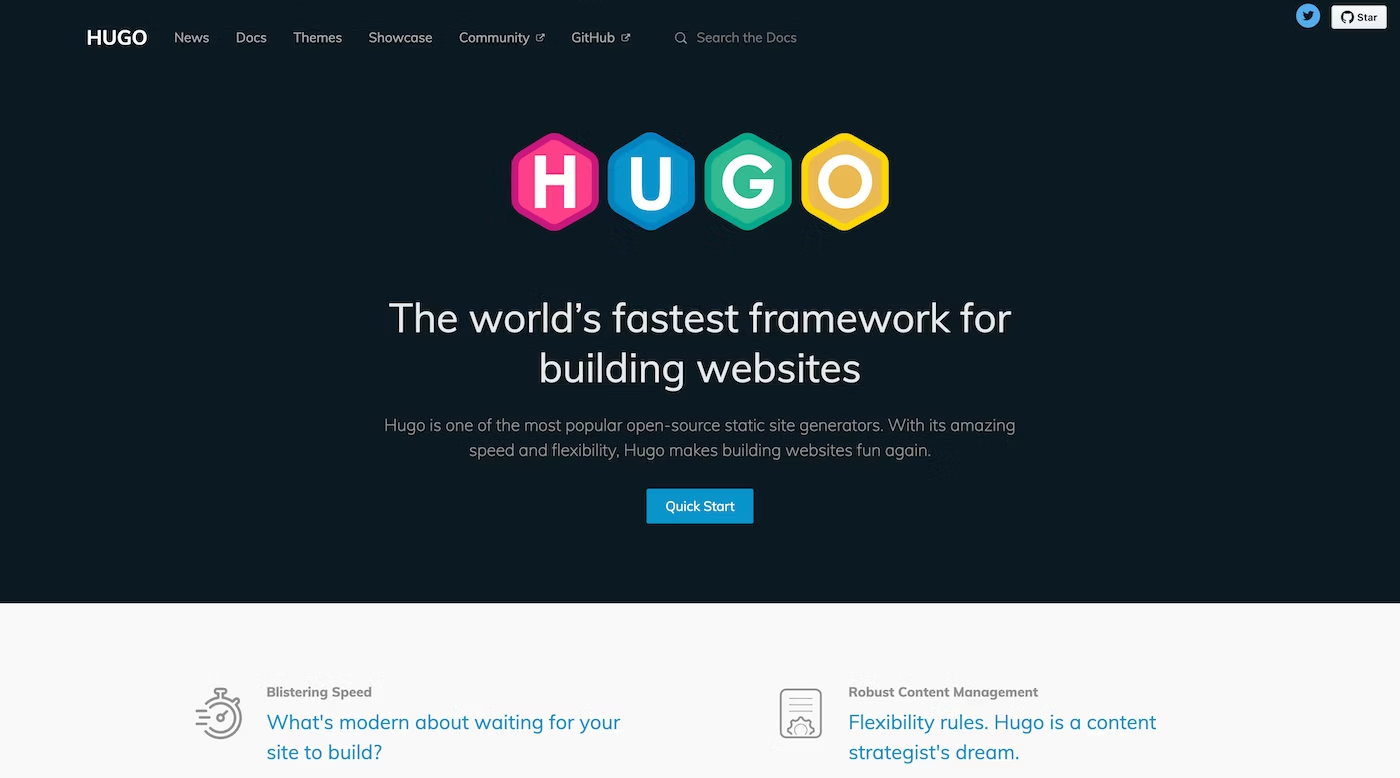
\includegraphics[width=6cm]{./image/02-chap3/hugo.png}
    \caption{hugoのホームページの写真}
    \label{chap3-hugo-image}
  \end{figure}

  \begin{tcolorbox}[title=hugoとは]
    HugoはGo言語で実装された「Webサイト構築フレームワーク」で、最初の公開は2013年という比較的新しいツールだ。コンテンツ管理システムではなく「Webサイト構築フレームワーク」と名乗っているとおり、コンテンツの管理ではなく、Webサイトで使われるHTMLファイルやRSSファイルなどの生成に特化した機能を備えている。
    \cite{hugoとは} \cite{hugo公式}
  \end{tcolorbox}

\section{GitHub Actions}

  \begin{figure}[H]
    \centering
    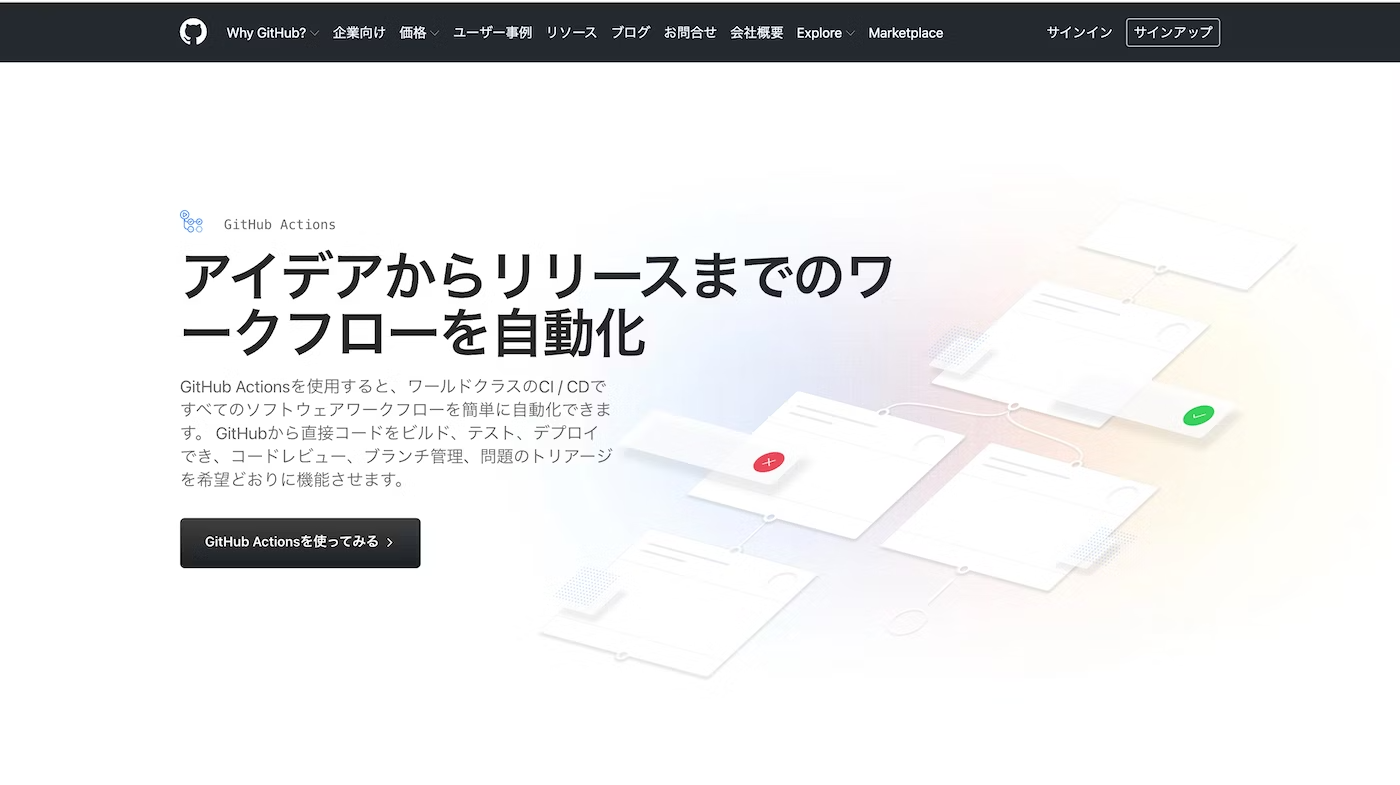
\includegraphics[width=6cm]{./image/02-chap3/githubActions.png}
    \caption{GitHub Actionsのホームページの写真}
    \label{chap3-githubAction-image}
  \end{figure}

  \begin{tcolorbox}[title=GitHub Pagesとは]
    GitHub Actionsで、ソフトウェア開発ワークフローをリポジトリの中で自動化し、カスタマイズし、実行しましょう。 CI/CDを含む好きなジョブを実行してくれるアクションを、見つけたり、作成したり、共有したり、完全にカスタマイズされたワークフロー中でアクションを組み合わせたりできます。
    \cite{githubAction}
  \end{tcolorbox}

\section{GitHub Pages}

  \begin{tcolorbox}[title=hugoとは]
    GitHub Pages は、GitHub のリポジトリから HTML、CSS、および JavaScript ファイル を直接取得し、任意でビルドプロセスを通じてファイルを実行し、ウェブサイトを公開できる静的なサイトホスティングサービスです。
    \cite{githubPages}
  \end{tcolorbox}


\section{CMS}

  \begin{tcolorbox}[title=CMSとは]
    「CMS」とは、「Contents Management System:コンテンツ・マネジメント・システム」の略で、簡単にいうとWebサイトのコンテンツを構成するテキストや画像、デザイン・レイアウト情報(テンプレート)などを一元的に保存・管理するシステムのことです。
    \cite{cmsとは}
  \end{tcolorbox}


\chapter{技術構成}
基本的には、esaによりマークダウンを作成して、それをGitHubに保存して、GitHub Actionsを用いてhugoに出力して、Webサイトに公開する方法です。

ほぼほぼノーコードでできる構成になっているので、そこまで手間がかからずに作成をすることができます。

\begin{figure}[H]
  \centering
  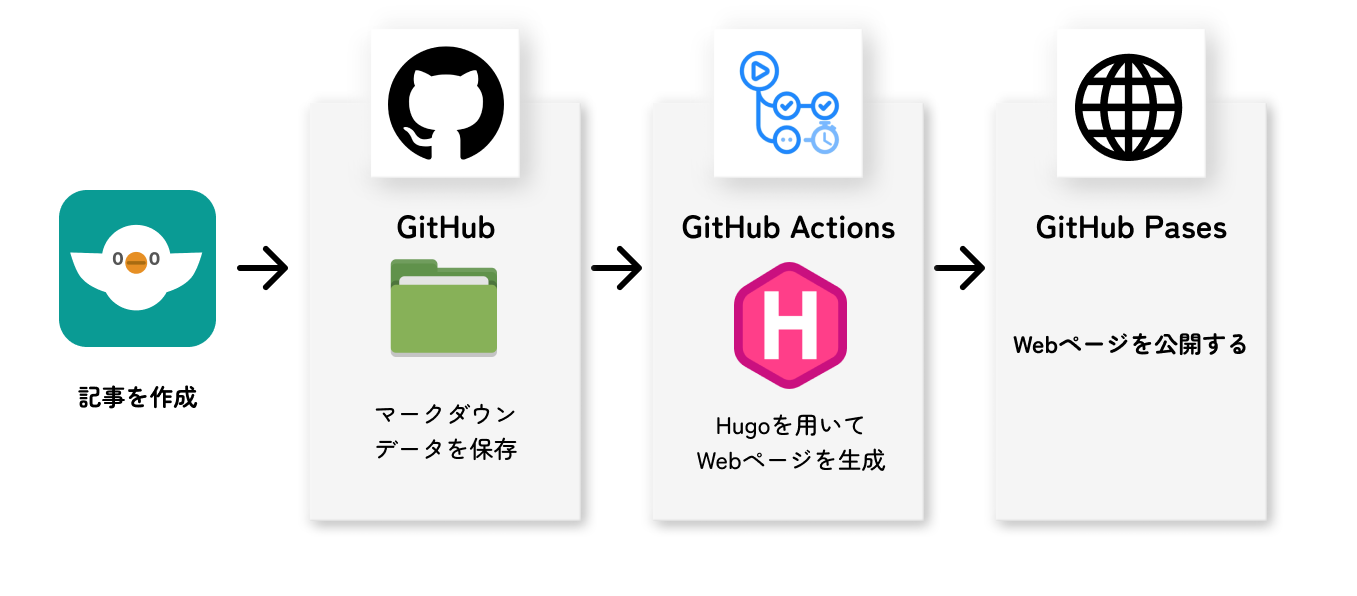
\includegraphics[width=14cm]{./image/02-chap4/flow.png}
  \caption{実際に用いた技術構成の図}
  \label{chap4-flow-image}
\end{figure}
\chapter{hugoについて}
hugoは静的なWebジェネレーターということで、軽く環境構築をしていきましょう。

\section{勉強資料}
  \url{https://youtu.be/hjD9jTi_DQ4}

\section{環境構築}
とりあえず、hugoをインストールしてみましょう。

  \begin{shaded}
    \begin{verbatim}
    $ brew install hugo
    \end{verbatim}
  \end{shaded}
  たったこれだけで完成です。

\section{hugoプロジェクト作成}
  あらかじめ、レポジトリを作成しておきましょう。
  GitHubからクローンをして、レポジトリを持ってきてください。

  \begin{shaded}
    \begin{verbatim}
    $ git clone 自分のリポジトリのURL

    $ cd クローンしたディレクトリ
    \end{verbatim}
  \end{shaded}

    では、次にhugoのプロジェクトを作成します。

  \begin{shaded}
    \begin{verbatim}
    $ hugo new site hugo-demo -f yml
    Congratulations! Your new Hugo site is created in 
    /Users/k22120kk/Downloads/hugo-demo.

    Just a few more steps and you're ready to go:

    1. Download a theme into the same-named folder.
      Choose a theme from https://themes.gohugo.io/ or
      create your own with the "hugo new theme <THEMENAME>" command.
    2. Perhaps you want to add some content. You can add single files
      with "hugo new <SECTIONNAME>/<FILENAME>.<FORMAT>".
    3. Start the built-in live server via "hugo server".

    Visit https://gohugo.io/ for quickstart guide and full documentation.
    \end{verbatim}
  \end{shaded}

  \begin{figure}[H]
    \centering
    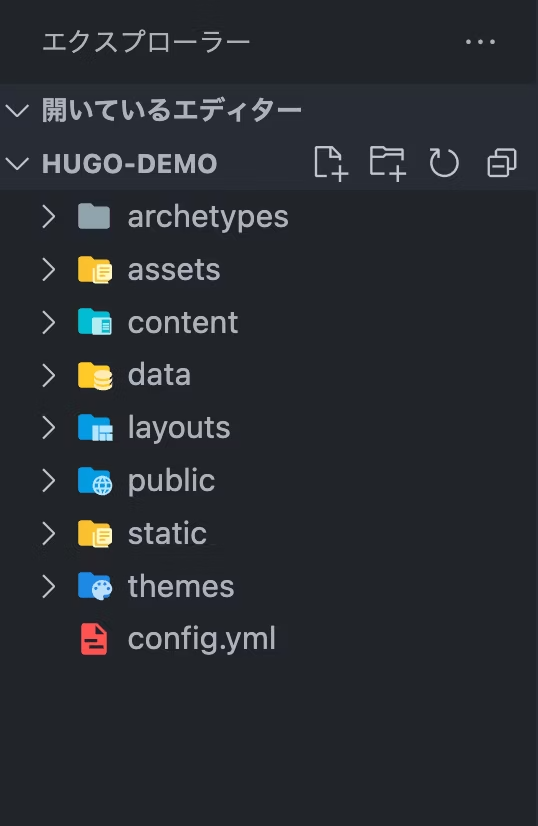
\includegraphics[width=8cm]{./image/02-chap5/filetree.png}
    \caption{実際に用いた技術構成の図}
    \label{chap5-firetree-image}
  \end{figure}

\section{テーマの設定}
  \subsection{テーマの選択}
    hugoではテーマを用いることで簡単にそれっぽいWebページを作成することができます。
    \url{https://themes.gohugo.io/}
    この中から気に入ったテーマを探してみてください。
    注意:テーマによって若干設定項目が変わる場所があるので気をつけてください。
    では今回は下記のテーマを用いて作成していこうと思います。
    \url{https://themes.gohugo.io/themes/hugo-theme-stack/}

    ちなみに、各テーマに大体ドキュメントがありますので、そのstartedなどをみることをお勧めします。
    今回のドキュメントはこちらになります。
    \url{https://stack.jimmycai.com/}

  \subsection{テーマの反映}
    では、ドキュメントの指示に従いながら、テーマの反映を行っていきます。
    \url{https://stack.jimmycai.com/guide/getting-started}

    cdを用いて、hugoのプロジェクトページまできてください。
    下記を実行することでテーマを反映させることができます。

    \begin{shaded}
      \begin{verbatim}
        $ git submodule add https://github.com/CaiJimmy/hugo-theme-stack/
        themes/hugo-theme-stack
      \end{verbatim}  
    \end{shaded}

    git initをしていない場合はこちらで実行してみてください。

    \begin{shaded}
      \begin{verbatim}
        $ git clone https://github.com/CaiJimmy/hugo-theme-stack/
        themes/hugo-theme-stack
      \end{verbatim}  
    \end{shaded}
    
    そうすることにより、themesディレクトリが作成されて、テーマの素材が入ります。

    \begin{figure}[H]
      \centering
      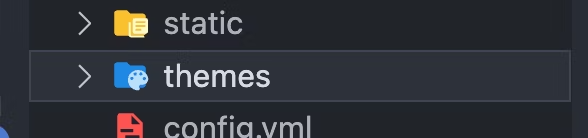
\includegraphics[width=8cm]{./image/02-chap5/firetree-themes.png}
      \caption{themesフォルダーができている様子の図}
      \label{chap5-firetree-themes-image}
    \end{figure}

    では、configファイルを設定して、themeを設定しましょう

    \begin{tcolorbox}[breakable]
      \begin{verbatim}
        baseURL: ""
        languageCode: ja
        title: My New Hugo Site
        theme: hugo-theme-stack
      \end{verbatim}
    \end{tcolorbox}

    では、実際に動かしてみて、動作するか確認してみましょう。

    \begin{shaded}
      \begin{verbatim}
        $ hugo server
        Start building sites … 
        hugo v0.108.0+extended darwin/arm64 BuildDate=unknown
        WARN 2022/12/23 10:44:43 found no layout file for "HTML" for kind
         "taxonomy": You should create a template file which matches Hugo
          Layouts Lookup Rules for this combination.
        WARN 2022/12/23 10:44:43 found no layout file for "HTML" for kind
         "home": You should create a template file which matches Hugo 
         Layouts Lookup Rules for this combination.
        WARN 2022/12/23 10:44:43 found no layout file for "HTML" for kind
         "taxonomy": You should create a template file which matches Hugo
          Layouts Lookup Rules for this combination.

                          | EN  
        -------------------+-----
          Pages            |  3  
          Paginator pages  |  0  
          Non-page files   |  0  
          Static files     |  0  
          Processed images |  0  
          Aliases          |  0  
          Sitemaps         |  1  
          Cleaned          |  0  

        Built in 6 ms
        Watching for changes in /Users/k22120kk/Downloads/hugo-demo/
        {archetypes,assets,content,data,layouts,static}
        Watching for config changes in /Users/k22120kk/Downloads/
        hugo-demo/config.yml
        Environment: "development"
        Serving pages from memory
        Running in Fast Render Mode. For full rebuilds on change: 
        hugo server --disableFastRender
        Web Server is available at http://localhost:1313/ 
        (bind address 127.0.0.1)
        Press Ctrl+C to stop
      \end{verbatim}  
    \end{shaded}

    ウェブブラウザでhttp://localhost:1313/ をURLに入れて読み込んでみましょう。

    下のような画像が出力されれば成功です。

    \begin{figure}[H]
      \centering
      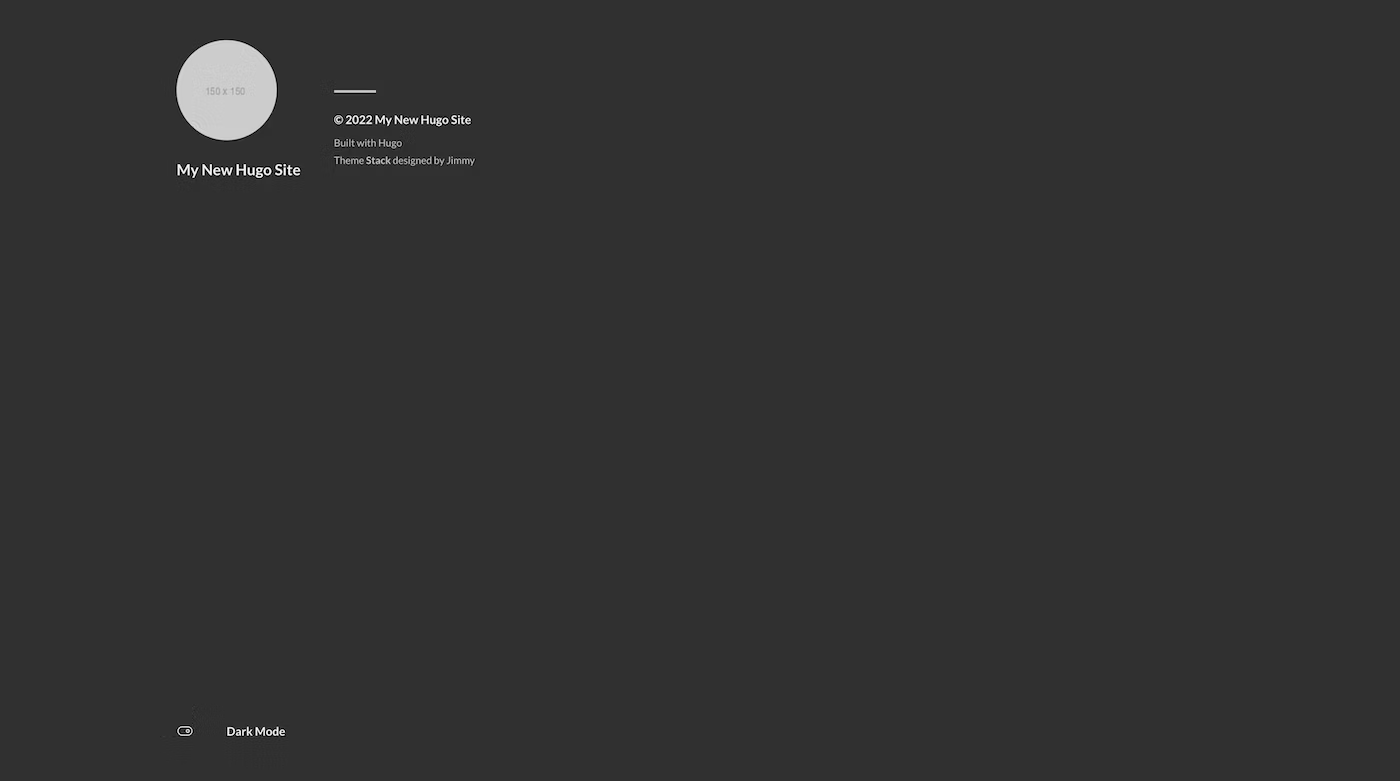
\includegraphics[width=8cm]{./image/02-chap5/output-homepage.png}
      \caption{テーマが反映された様子の図}
      \label{chap5-homepage-image}
    \end{figure}

  \subsection{Webページを作成してみる}
    では、軽くマークダウンを作成をしてWebページを作成してみましょう
    下のコマンドを入力して、マークダウンを作成してみましょう。

    \begin{shaded}
      \begin{verbatim}
       $ hugo new post/first.md
      \end{verbatim}
    \end{shaded}

    そうすると下記のようなファイルができているはずです。
    
    \begin{tcolorbox}[breakable]
      \begin{verbatim}
        ---
        title: "First"
        date: 2022-12-23T10:49:46+09:00
        draft: true
        ---
      \end{verbatim}
    \end{tcolorbox}

    それでは追加で書き加えてみます。
    ここで状態が編集モードになっているため、draft:trueをdraft:falseに変更しましょう。
    こうしないと、デプロイした時に表示されなくなります。

    \begin{tcolorbox}[breakable]
      \begin{verbatim}
        ---
        title: "First"
        date: 2022-12-23T10:49:46+09:00
        draft: false
        ---

        # 最初の書き込みです
        ここから僕だけのウェブサイトが生まれます。
      \end{verbatim}
    \end{tcolorbox}

    下のように、作成したWebページが作られているはずです。

    \begin{figure}[H]
      \centering
      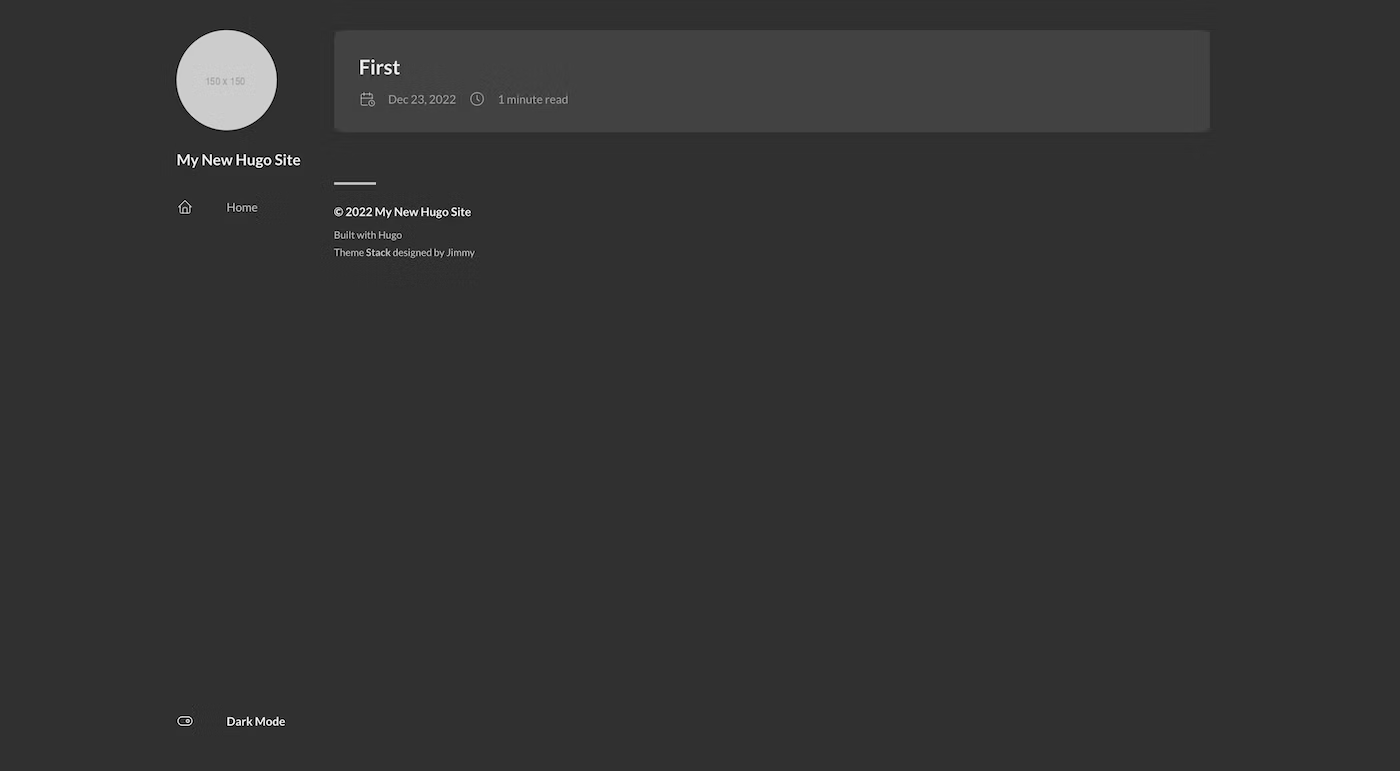
\includegraphics[width=8cm]{./image/02-chap5/add-file-list.png}
      \caption{ファイルが追加されている様子の図}
      \label{chap5-add-file-list-image}
    \end{figure}

    \begin{figure}[H]
      \centering
      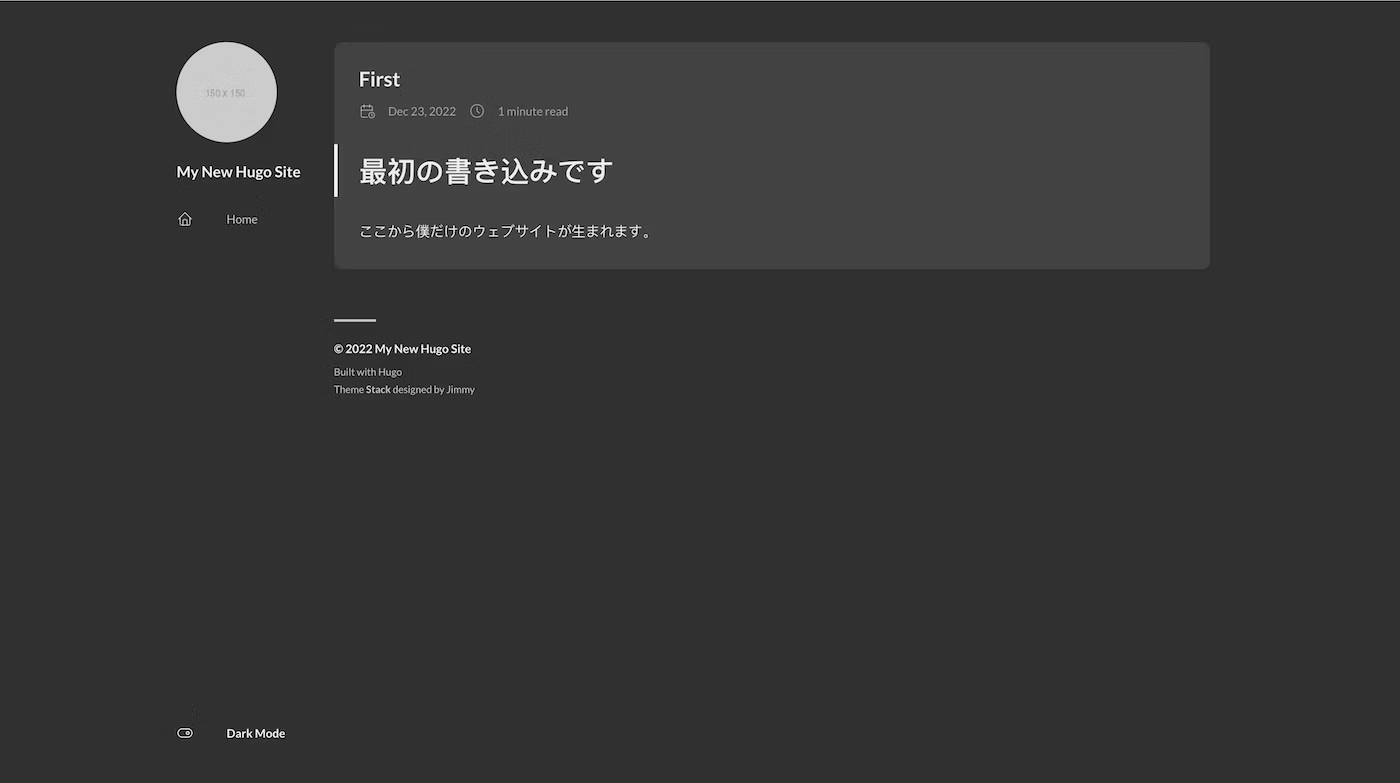
\includegraphics[width=8cm]{./image/02-chap5/add-file-content.png}
      \caption{ファイルの中身が追加されている様子の図}
      \label{chap5-add-file-content-image}
    \end{figure}

  \subsection{細かい設定など}
    ここでは、細かく説明はしませんが、configファイルや、mdファイルの上の部分で様々な設定をすることができます。
    詳しい説明をしてくれているWebページを紹介しますので、ぜひご自身で色々触って自分だけのオリジナルサイトを作ってみてください。

    \subsubsection{configの設定}
      \url{https://github.com/CaiJimmy/hugo-theme-stack/blob/master/exampleSite/config.yaml}

      \url{https://miiitomi.github.io/p/hugo/}

    \subsubsection{フロントマターの設定}
      \url{https://takaken.tokyo/dev/hugo/post/write-post/}

    




    
  



\chapter{githubpagesの設定(デプロイをする)}
\section{gitmodulesの設定}

  \begin{tcolorbox}[title=gitmodulesとは]
    Git サブモジュールは、あるリポジトリの内容を別のリポジトリ内に含めることを、参照されるリポジトリの場所を指定するだけでできるようになる Git SCMの機能です。 
    
    これは、外部ライブラリのソースをアプリケーションのソースツリーに含めるメカニズムを提供します。
    引用:\url{https://devcenter.heroku.com/ja/articles/git-submodules#:~:text=Git%20%E3%82%B5%E3%83%96%E3%83%A2%E3%82%B8%E3%83%A5%E3%83%BC%E3%83%AB%E2%80%8B%E3%81%AF,%E3%83%A1%E3%82%AB%E3%83%8B%E3%82%BA%E3%83%A0%E3%82%92%E6%8F%90%E4%BE%9B%E3%81%97%E3%81%BE%E3%81%99%E3%80%82}

  \end{tcolorbox}

  ということで、デプロイする時に、この設定をしないとエラーが発生するので、設定をしましょう

  \begin{shaded}
    \begin{verbatim}
    $ touch .gitmodules
    \end{verbatim}
  \end{shaded}

  \begin{figure}[H]
    \centering
    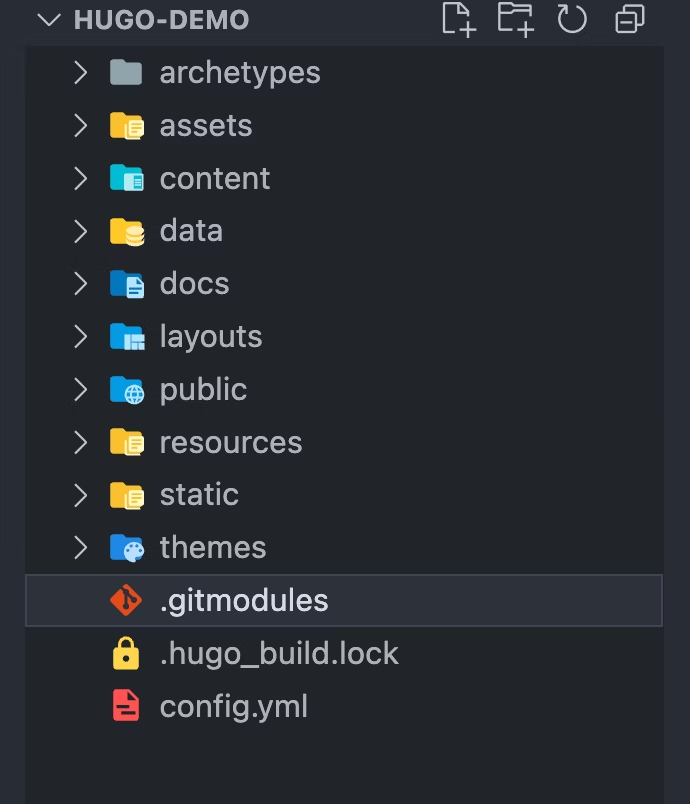
\includegraphics[width=8cm]{./image/02-chap6/make-modules-tree.png}
    \caption{GitModuleを作った時のTree構造}
    \label{chap6-make-modules-tree-image}
  \end{figure}

  テーマによって、設定内容が変わってくるので、テーマに合わせた設定にしてください。

  \begin{tcolorbox}[breakable]
    \begin{verbatim}
      [submodule "themes/hugo-theme-stack"]
      path = themes/hugo-theme-stack
      url = https://github.com/CaiJimmy/hugo-theme-stack
    \end{verbatim}
  \end{tcolorbox}

\section{baseurlの設定}

  あとはbaseURLを指定しましょう。
  ここが正しくないと、CSSがうまいこと読み取られないなどのバグが発生します。

  ということで、configファイルを編集しましょう。

  今回は、自分の設定をそのまま表示させていますが、カスタムドメインを使っていない場合は、https://githubのユーザー名.github.io/レポジトリ名/と設定しましょう。
  カスタムドメインを使用している場合は、設定したドメインをそのまま書き込んでください。

  \begin{tcolorbox}[breakable]
    \begin{verbatim}
      baseURL: "https://harutiro.github.io/hugo_test_qiita/"
      languageCode: ja
      title: My New Hugo Site
      theme: hugo-theme-stack
      publishDir: "docs"

      menu:
          main:
            - identifier: home
              name: Home
              url: /
              params:
                icon: home
    \end{verbatim}
  \end{tcolorbox}

\section{静的なファイルを生成する}

  それでは、githubpagesの公開をするために、静的なファイルを生成します。
  生成する時にdocsに作ってもらえると都合がいいので、configを設定しておきましょう。

  publishDir: "docs"を追記してあげてください。

  \begin{tcolorbox}[breakable]
    \begin{verbatim}
      baseURL: ""
      languageCode: ja
      title: My New Hugo Site
      theme: hugo-theme-stack
      publishDir: "docs"

      menu:
          main:
            - identifier: home
              name: Home
              url: /
              params:
                icon: home
    \end{verbatim}
  \end{tcolorbox}


  あとは下記のコマンドを打ち込んで静的なファイル(html,cssなど)を作成しましょう


  \begin{shaded}
    \begin{verbatim}
    $ hugo
    \end{verbatim}
  \end{shaded}

  \begin{figure}[H]
    \centering
    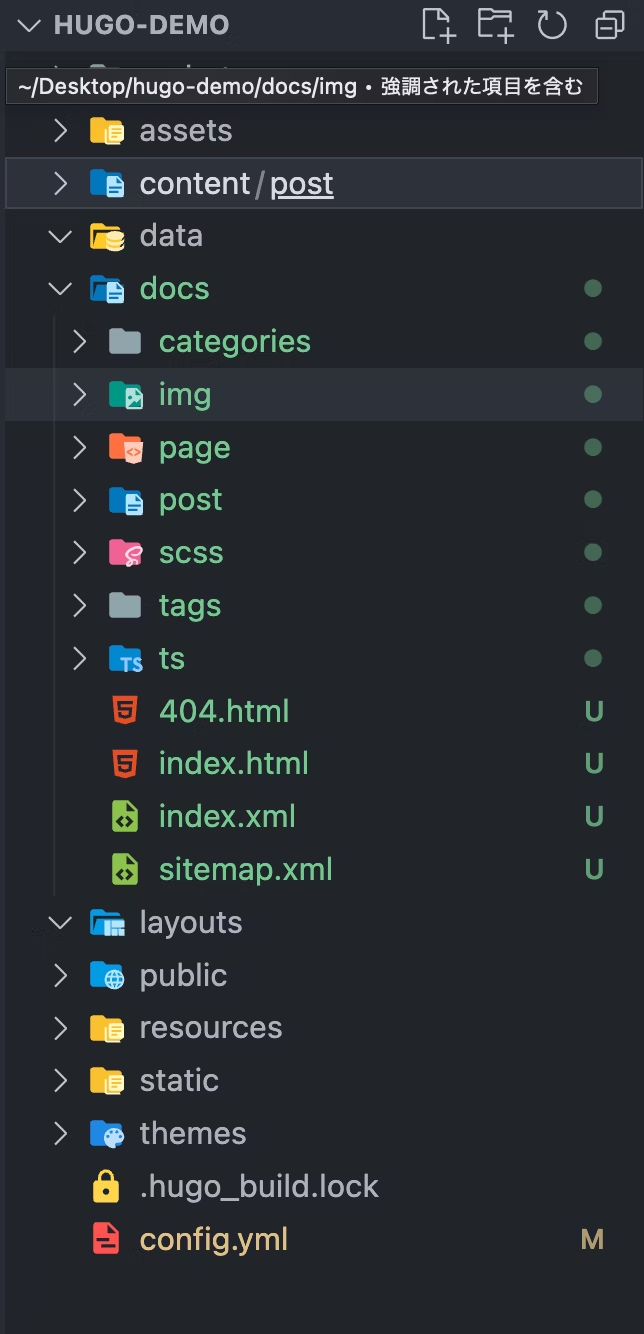
\includegraphics[width=6cm]{./image/02-chap6/docs-genelate.png}
    \caption{docsに静的なファイルが生成された図}
    \label{chap6-docs-genelate-image}
  \end{figure}

\section{github pagesの設定をする}

  それでは、githubを用いてデプロイを行ってみましょう。
  とりあえず、いつもの手順でgithubに公開しましょう。

  \begin{shaded}
    \begin{verbatim}
    $ git init
    $ git add -A
    $ git commit -m "initalCommit"
    $ git remote add origin 個人のレポジトリ
    $ git push origin master
    \end{verbatim}
  \end{shaded}

  \begin{figure}[H]
    \centering
    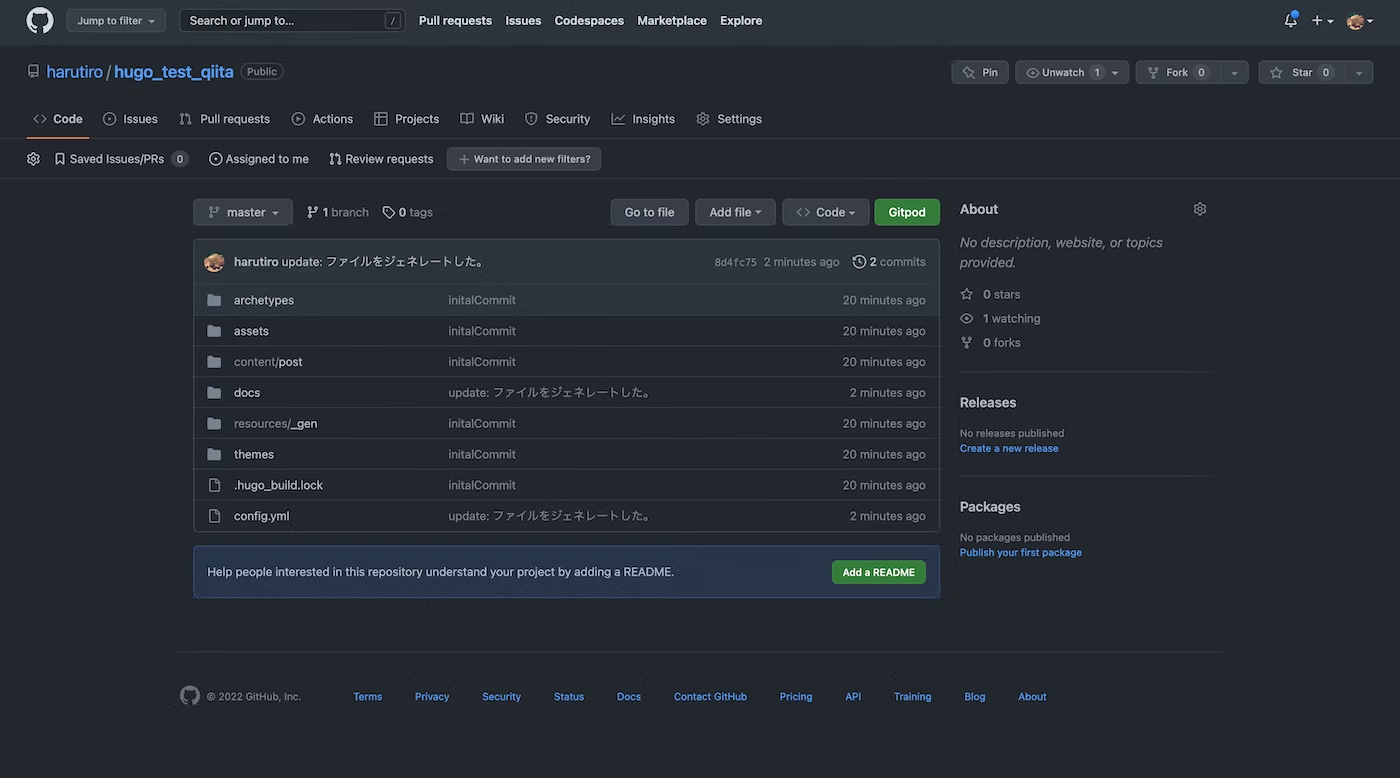
\includegraphics[width=8cm]{./image/02-chap6/git1.png}
    \caption{レポジトリが作成された様子}
    \label{chap6-git1-image}
  \end{figure}

  それでは、pagesの設定をしていきましょう。
  setting/pagesを開きましょう。

  \begin{figure}[H]
    \centering
    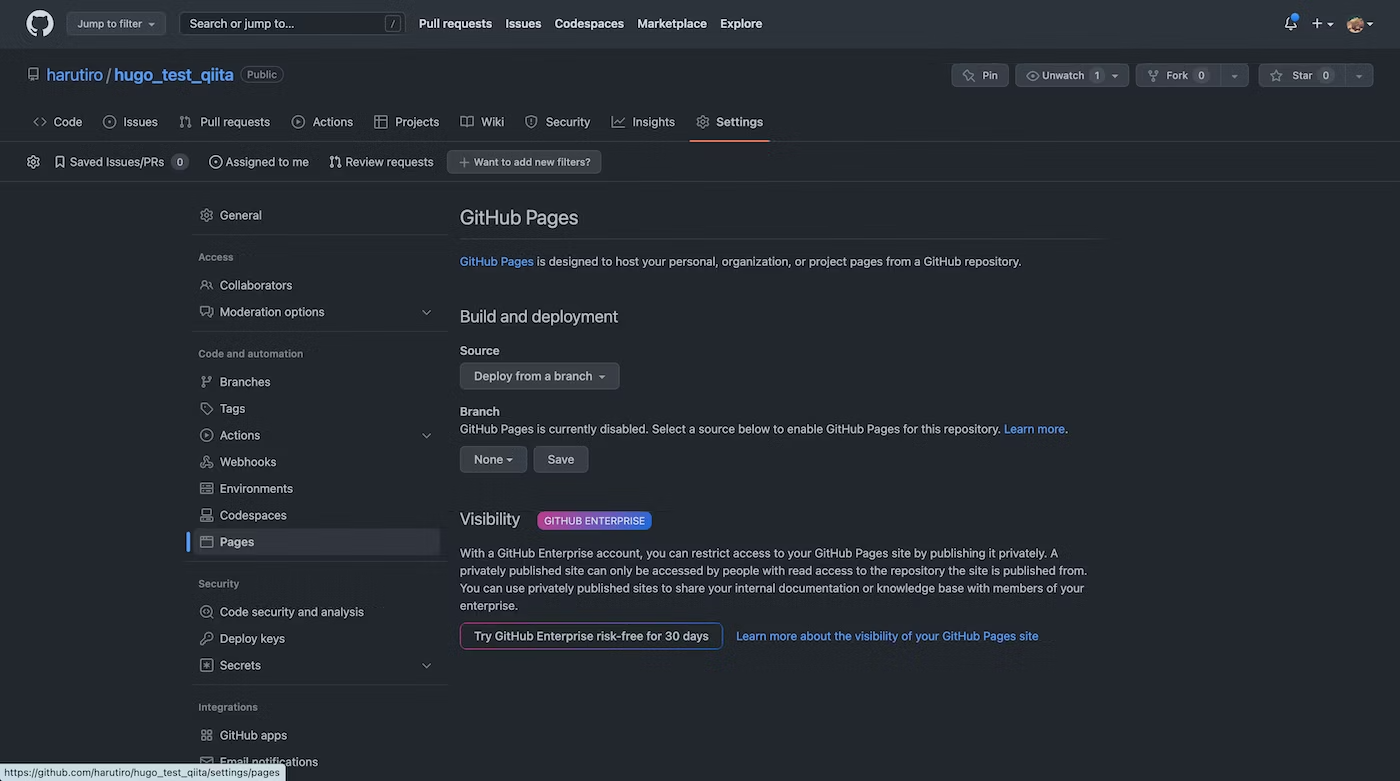
\includegraphics[width=8cm]{./image/02-chap6/git2.png}
    \caption{pagesの設定画面}
    \label{chap6-pages1-image}
  \end{figure}

  sourceをDeploy from a branchに設定して
  Branchをmaster /docsに設定しましょう

  カスタムドメインは今回は説明しません。
  これで、masterにデプロイして、しばらく待つとデプロイが始まります。

  \begin{figure}[H]
    \centering
    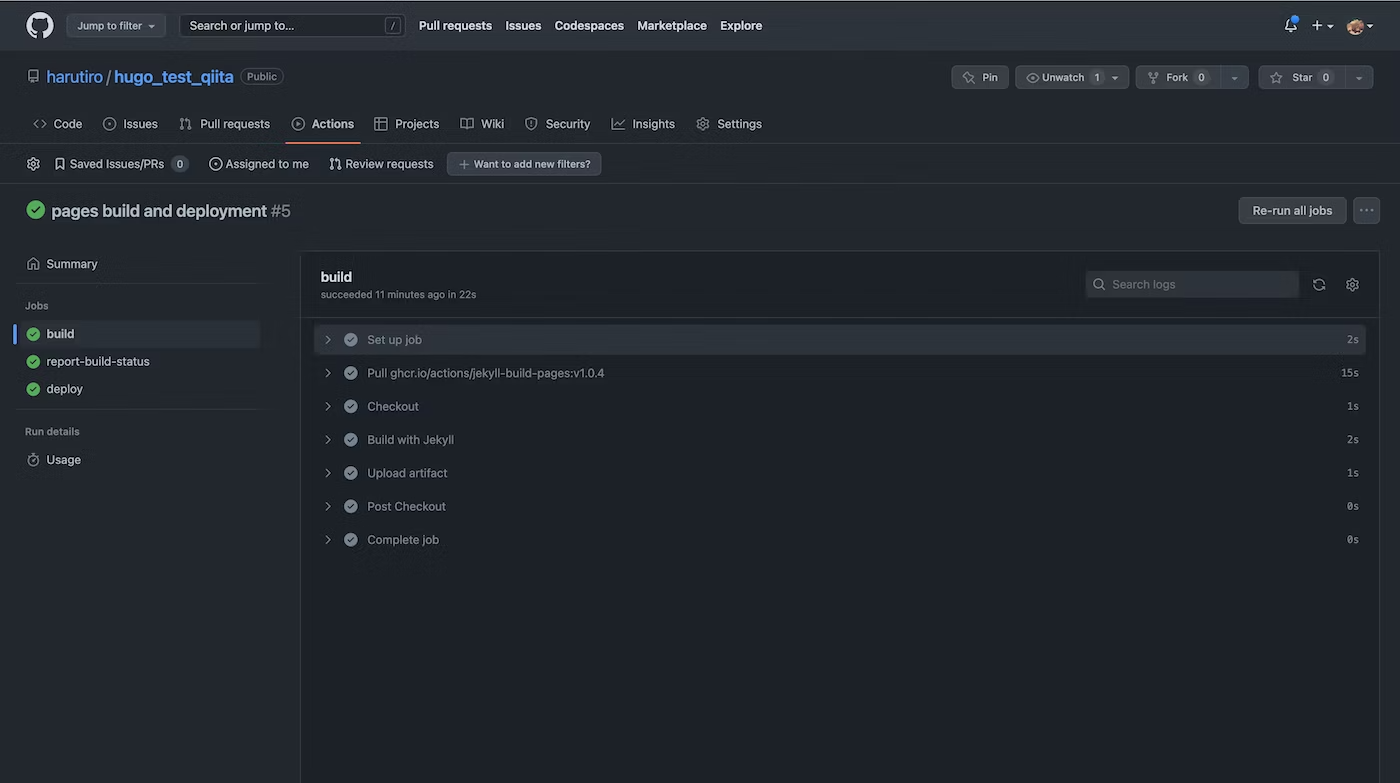
\includegraphics[width=8cm]{./image/02-chap6/git4.png}
    \caption{デプロイが始まった様子}
    \label{chap6-pages2-image}
  \end{figure}

  うまくいった場合、設定したbaseURLの場所に行くとうまく表示されているはずです。

  \begin{figure}[H]
    \centering
    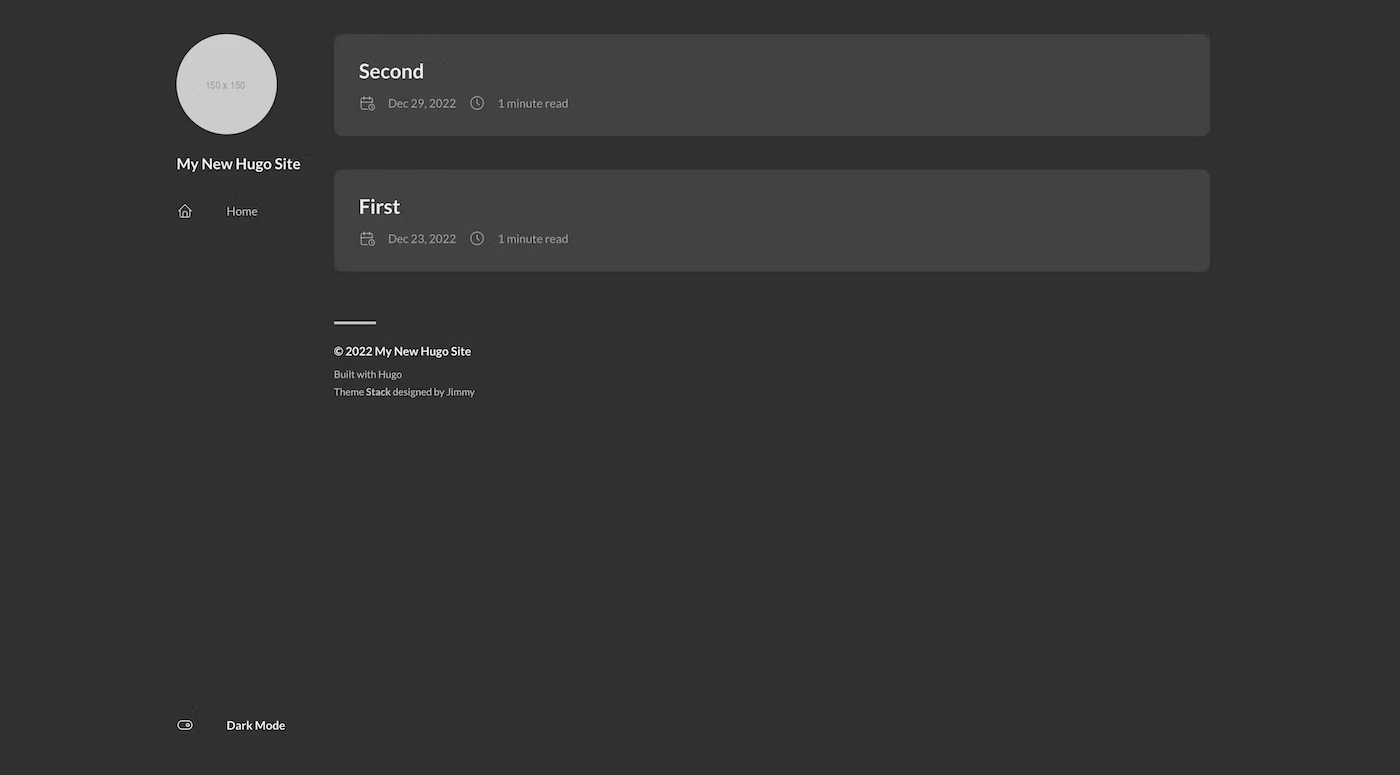
\includegraphics[width=8cm]{./image/02-chap6/view_hugo.png}
    \caption{公開がうまくいった様子}
    \label{chap6-pages3-image}
  \end{figure}




\chapter{esaについて}

esaではいつかのアップデートで、直接GitHubに記事を保存ができるようになりました。
2016年のアップデートらしいですね。
細かい設定などは下の記事でご確認ください。

\url{https://docs.esa.io/posts/176}

では、とりあえず設定をしていきましょう。

\section{設定}

  まずは、esaの設定をしましょう。
  
  \begin{figure}[H]
    \centering
    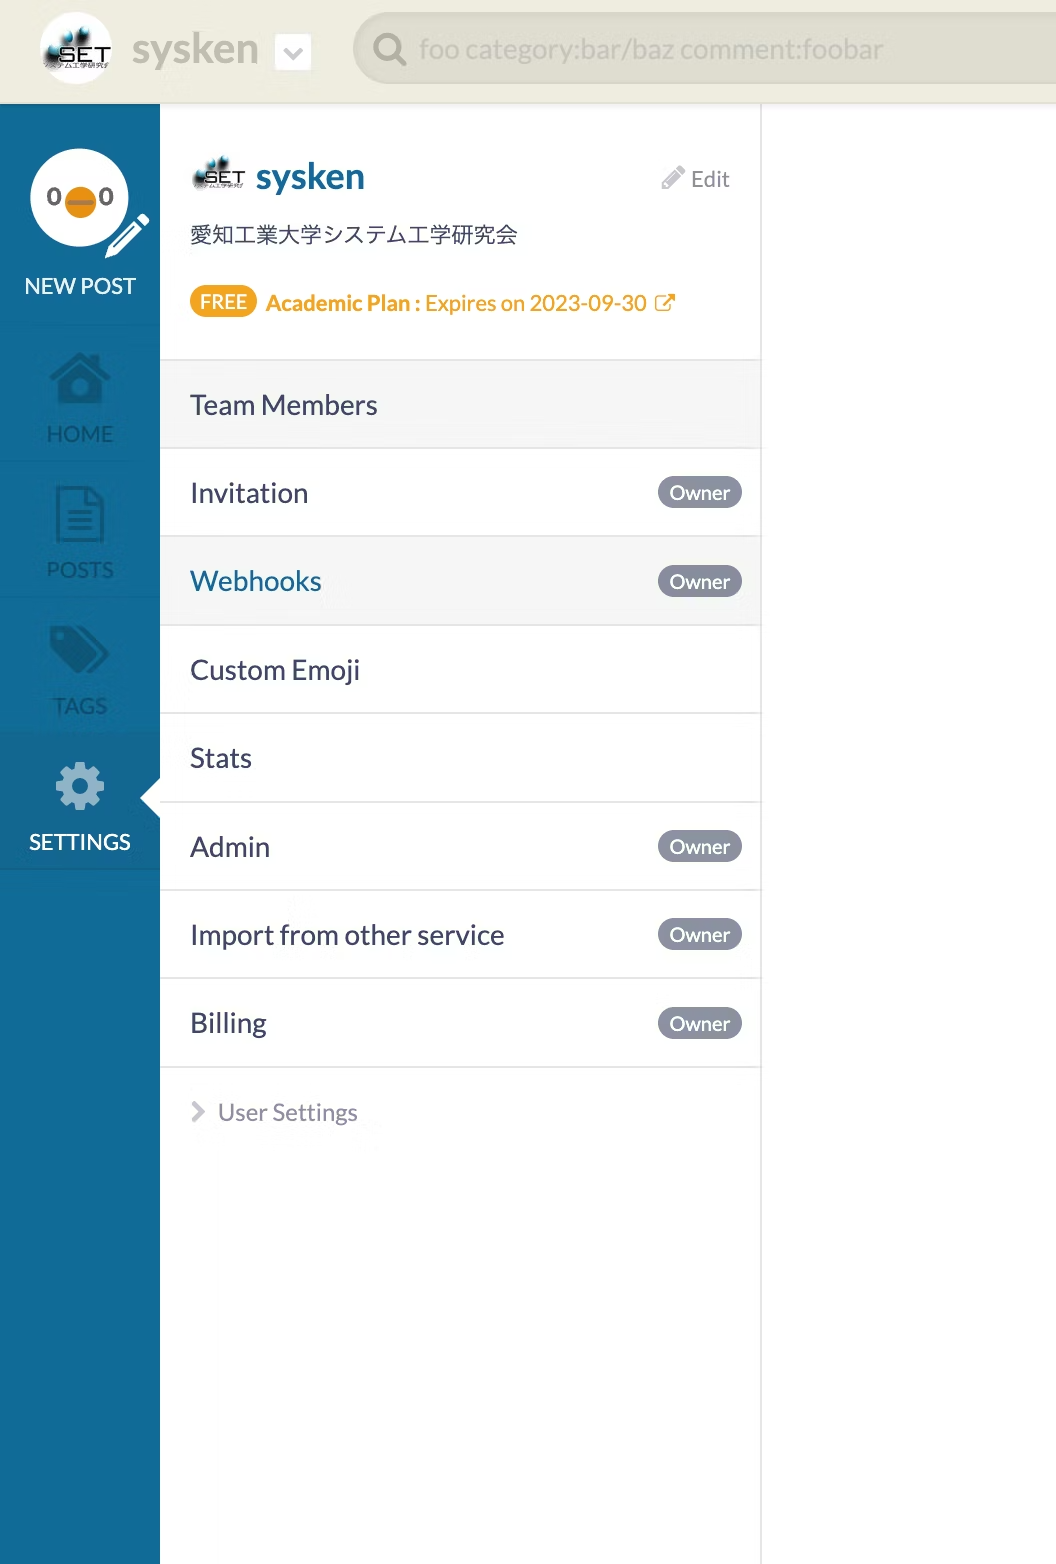
\includegraphics[width=8cm]{./image/02-chap7/esa-setting.png}
    \caption{esaの設定画面}
    \label{chap7-esa-setting-image}
  \end{figure}

  setting - Webhooksを選択します。

  addを選択して、GitHub(β)を選択します。 

  \begin{figure}[H]
    \centering
    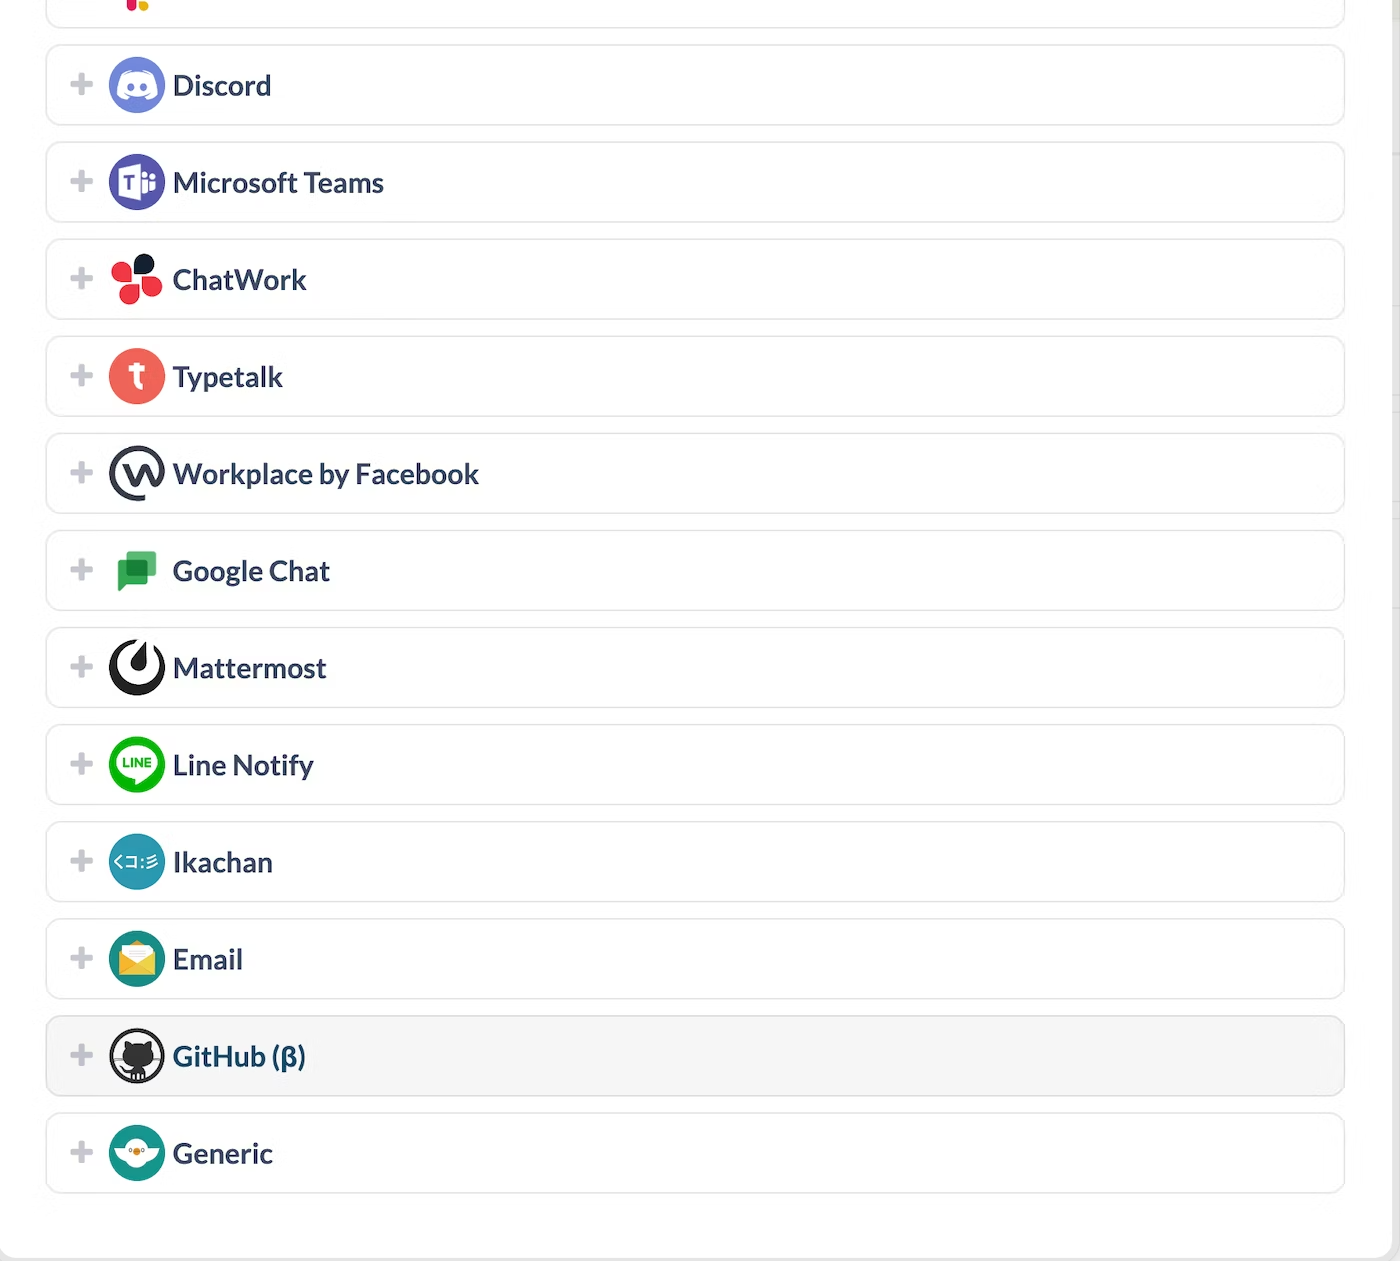
\includegraphics[width=8cm]{./image/02-chap7/esa-setting-list.png}
    \caption{esaの設定画面 API連携の部分 }
    \label{chap7-esa-setting-list-image}
  \end{figure}

  あとは、様々な設定を行って、保存をします。

  esa root category
  ここで、Webページに更新されて欲しい記事のディレクトリを選択することもできるので設定してみてください。
  output directory
  出力の場所はHugoの関係で指定しないといけないので、/content/post/と設定しましょう。

  \begin{figure}[H]
    \centering
    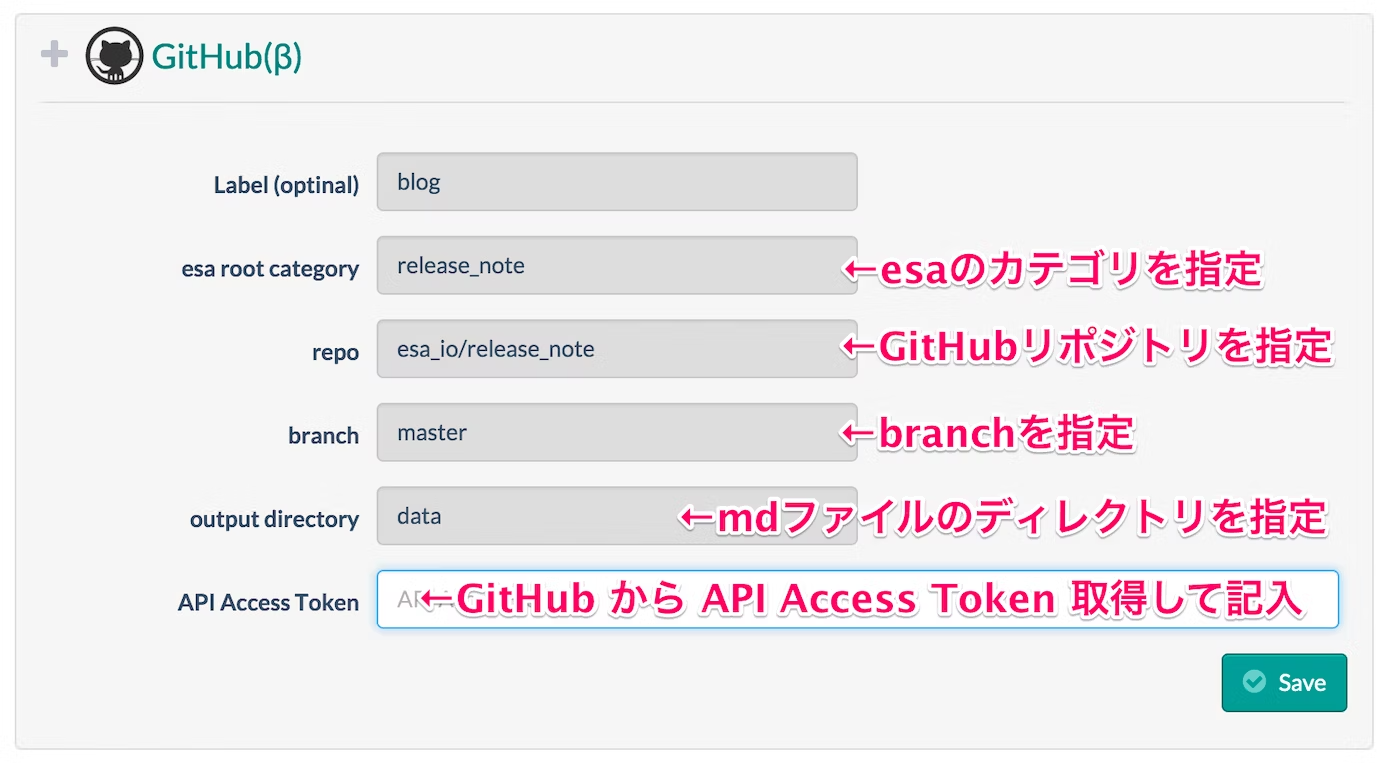
\includegraphics[width=8cm]{./image/02-chap7/github-setting.png}
    \caption{esaの設定画面 GitHubの設定 }
    \label{chap7-github-setting-image}
  \end{figure}

  \begin{figure}[H]
    \centering
    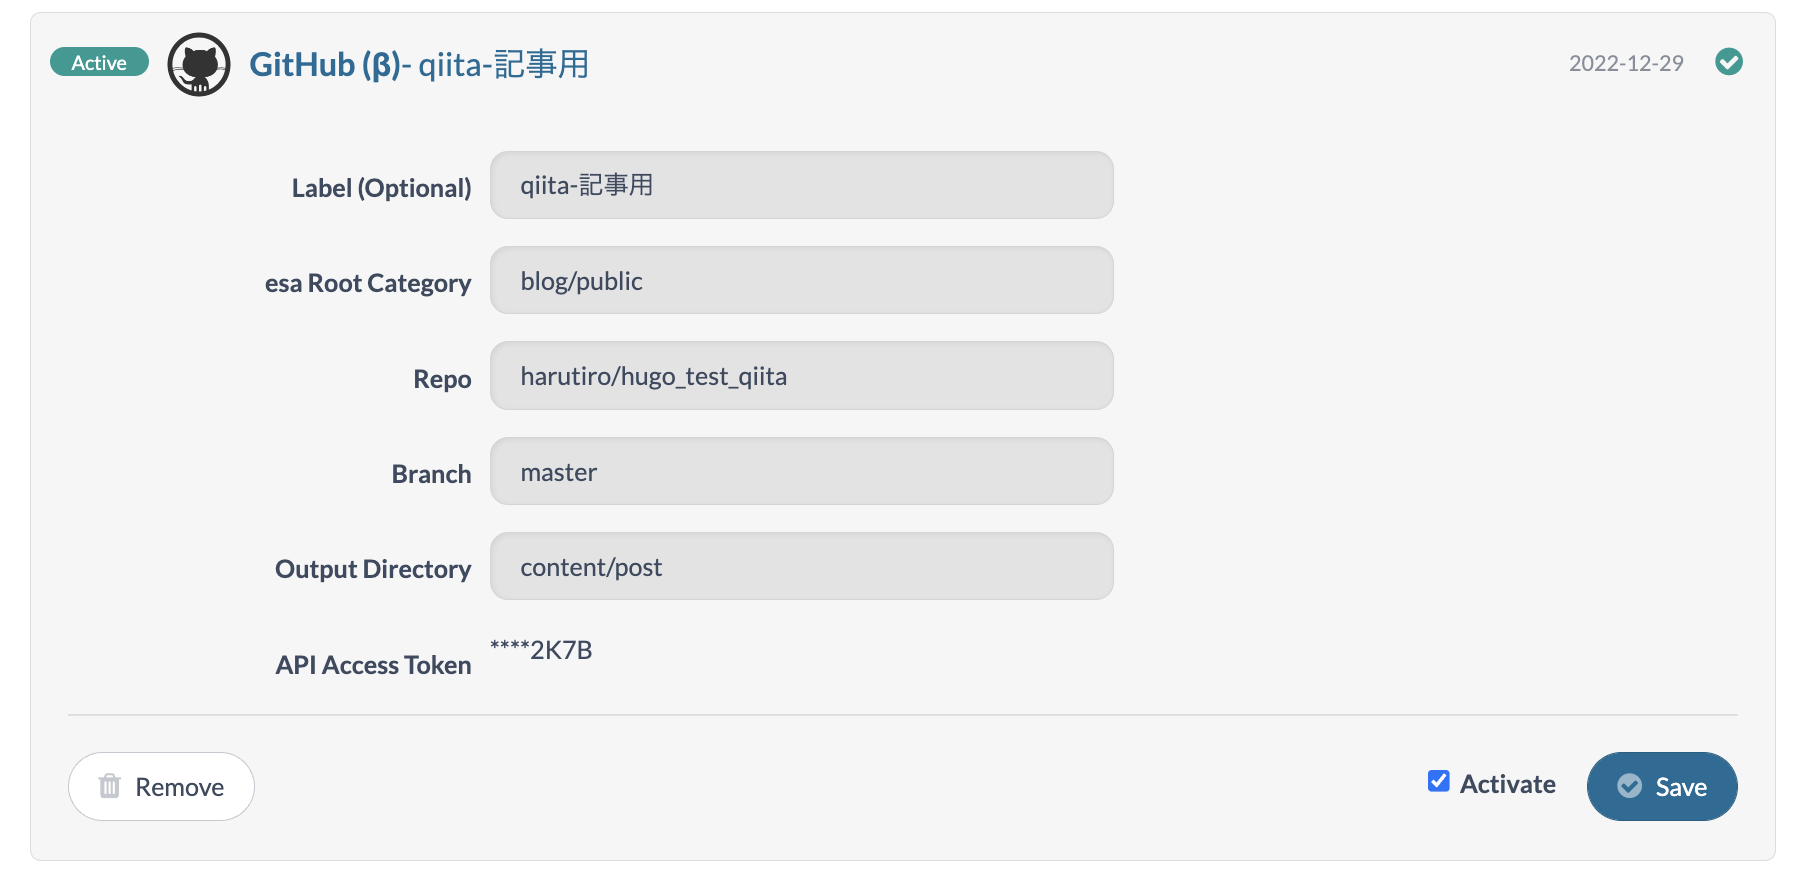
\includegraphics[width=8cm]{./image/02-chap7/github-setting-writed.png}
    \caption{esaの設定画面 GitHubの設定 実際の設定項目 }
    \label{chap7-github-setting-writed-image}
  \end{figure}

  これで記事が更新(新規)で作られたら、GitHubのレポジトリの更新されました。

  では、実際にesaが更新されたらpostに新しいファイルが追加されるか確認してみましょう。

  こういったファイルを投稿してみました。

  \begin{figure}[H]
    \centering
    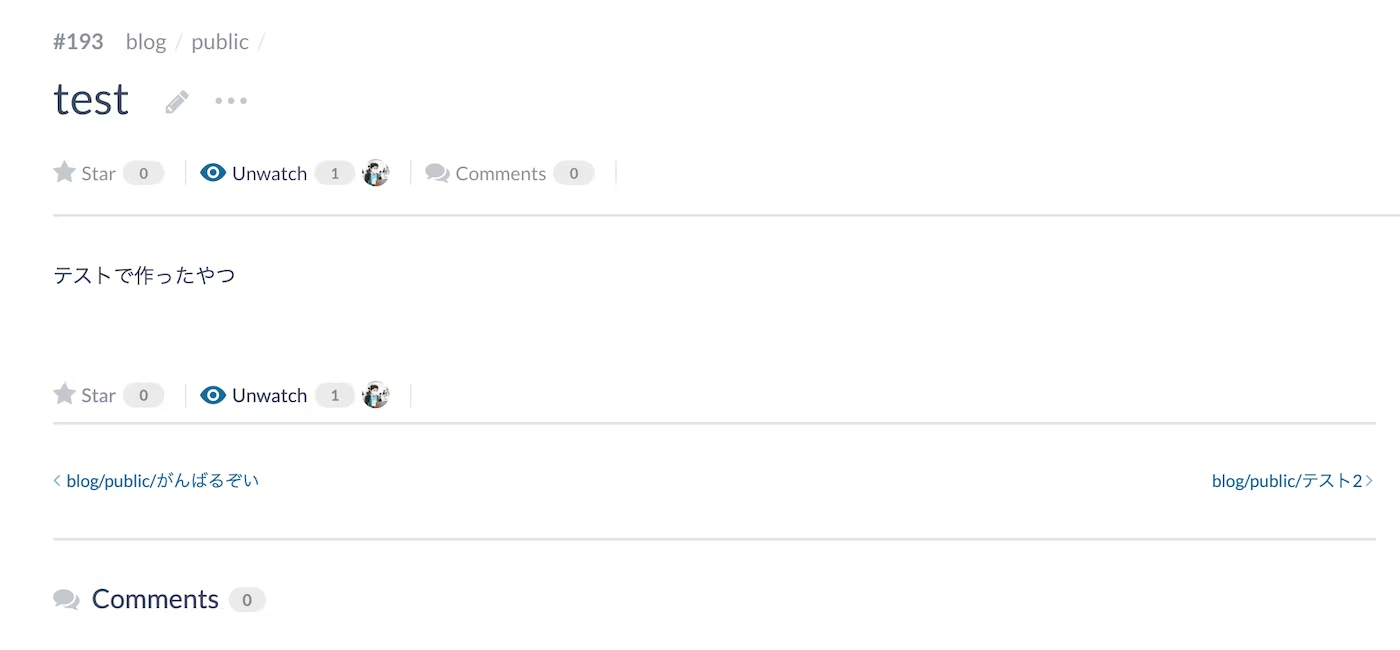
\includegraphics[width=8cm]{./image/02-chap7/esa-posted.png}
    \caption{esaに投稿した記事 }
    \label{chap7-esa-posted-image}
  \end{figure}

  ファイルが新しく追加されてますね。

  \begin{figure}[H]
    \centering
    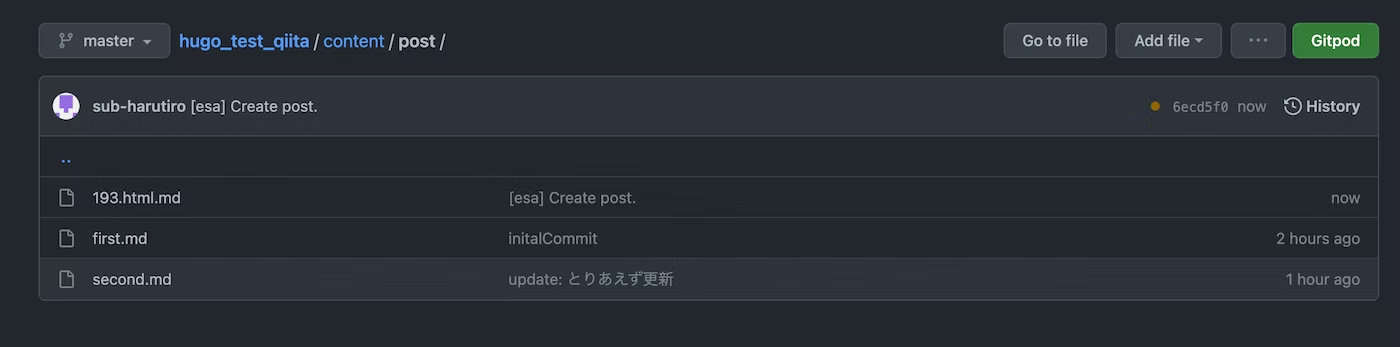
\includegraphics[width=8cm]{./image/02-chap7/github-upload-image.png}
    \caption{GitHubに記事が追加された }
    \label{chap7-github-upload-image-image}
  \end{figure}

  しかし、このままだとWebページは更新されていません。
  それはHugoを用いて静的なファイルを生成していないためです。

  では次の章ではGitHub Actionsを用いてHugoを実行するプログラムを書いていきましょう。




  
  
  
\chapter{GitHub Actionsの設定}

GitHub Actionsを設定していきましょう。

流れとしては、新しいブランチを作成して、その中にHugoを実行させて静的なファイルを作成して、強制プッシュを用いて更新をかけていくやり方です。
無理くり動かしている雰囲気は感じますが、今はこのままでいきましょう。
何かいい方法がありましたら、教えてください。

.github/workflowsフォルダーを作成しましょう
その中にgithub-actions-demo.ymlとして、ファイルを作成しておきましょう

\begin{shaded}
  \begin{verbatim}
  $ mkdir .github
  $ cd .github
  $ mkdir workflows
  $ cd workflows
  $ touch github-actions-demo.yml
  \end{verbatim}
\end{shaded}

\begin{figure}[H]
  \centering
  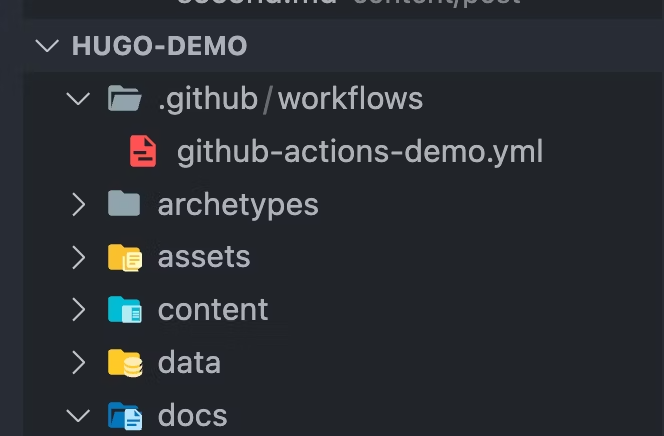
\includegraphics[width=8cm]{./image/02-chap8/make-github-workflow.png}
  \caption{GitHub Actionsの設定ファイルを作成 }
  \label{chap8-make-github-workflow-image}
\end{figure}

中のファイルはこのように書き込んでいきましょう。
一部人によって変わる場所があるので気をつけてください。

** 変えるもの **
起爆させるブランチ名 コミットする時のユーザー名、ファイル名

\begin{tcolorbox}[breakable]
  \begin{verbatim}
    name: Deploy Sakura Server

    on:
      push:
        branches:
          - master  # masterブランチが更新された時に発火させる
    
    jobs:
      deploy:
        name: deploy
        runs-on: ubuntu-latest
        
        steps:
          - uses: actions/checkout@v2
            with:
              submodules: true  # Fetch Hugo themes 
(true OR recursive)
              fetch-depth: 0    # Fetch all history for .
GitInfo and .Lastmod
    
          - name: Setup Hugo
            uses: peaceiris/actions-hugo@v2
            with:
              hugo-version: '0.102.3'  # コンパイルに使用するHugoのバージョンを指定
    
          - name: Build
            run: hugo --minify  # 実際にHugoでコンパイルする(--minifyはファイルを圧縮するオプション)
    
          - name: git commit
            uses: EndBug/add-and-commit@v9
            with:
              author_name: harutiro # 投稿するユーザーに合わせてください。
              author_email: hogehoge@example.com # 投稿するユーザーに合わせてください。
              new_branch: web_public
              message: 'hogehoge' # いい感じにメッセージを書いてあげてください。
              add: '* --force' 
              push: origin web_public --force
  \end{verbatim}
\end{tcolorbox}

あとは、新しくGitHub Pagesの設定を書き換えて完成です。
ブランチの位置をweb$\_$publicに書き換えましょう。

\begin{figure}[H]
  \centering
  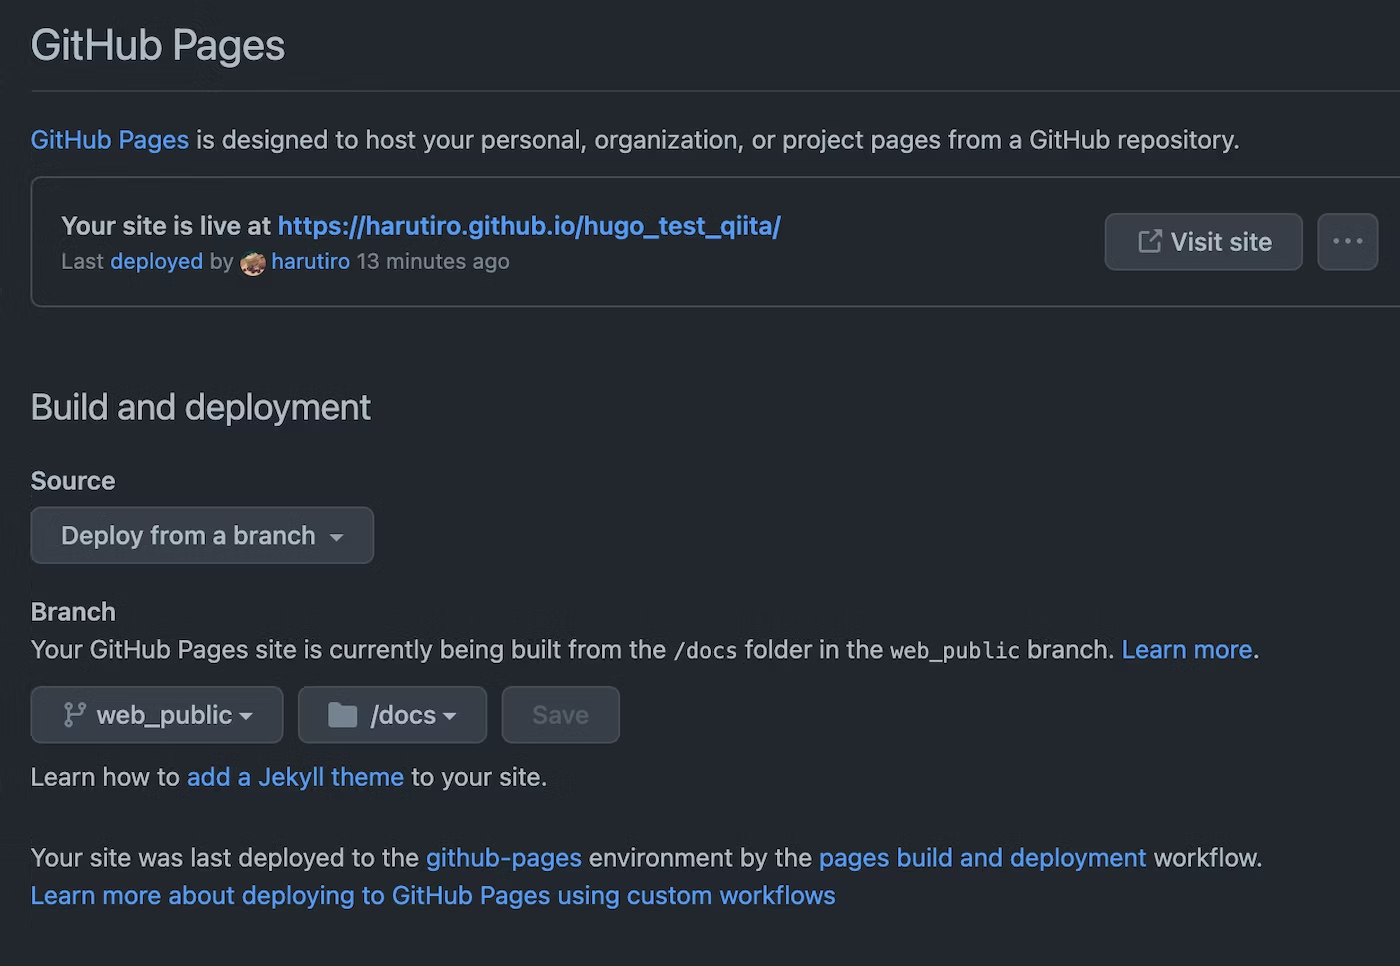
\includegraphics[width=8cm]{./image/02-chap8/web_public.png}
  \caption{GitHub Pagesの設定を書き換える}
  \label{chap8-web_public-image}
\end{figure}

これで完成です。
新しくpushがされたタイミングで更新がかかっていきます。
\chapter{動作実験}

\section{esaで記事を書く}
  今回はこの二つを投稿したとします。

  \begin{figure}[H]
    \centering
    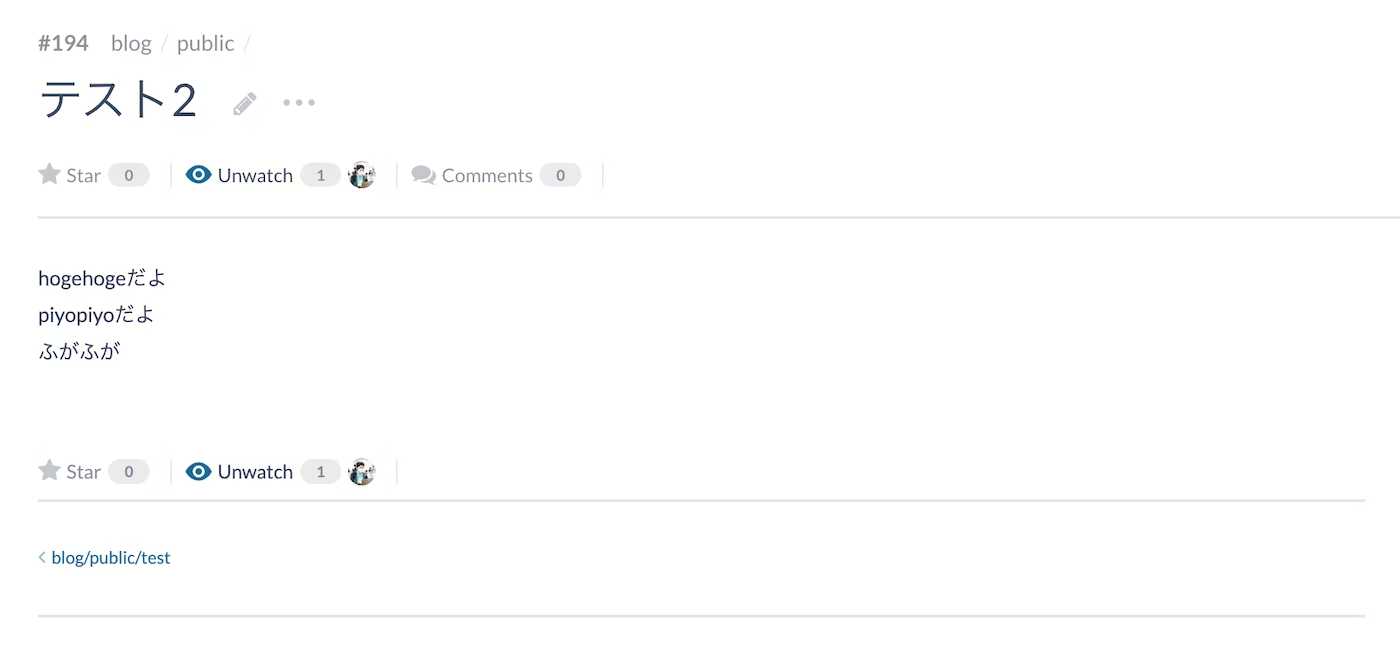
\includegraphics[width=8cm]{./image/02-chap9/esa-post-1.png}
    \caption{esaに投稿した記事1}
    \label{chap9-esa-post-1-image}
  \end{figure}

  \begin{figure}[H]
    \centering
    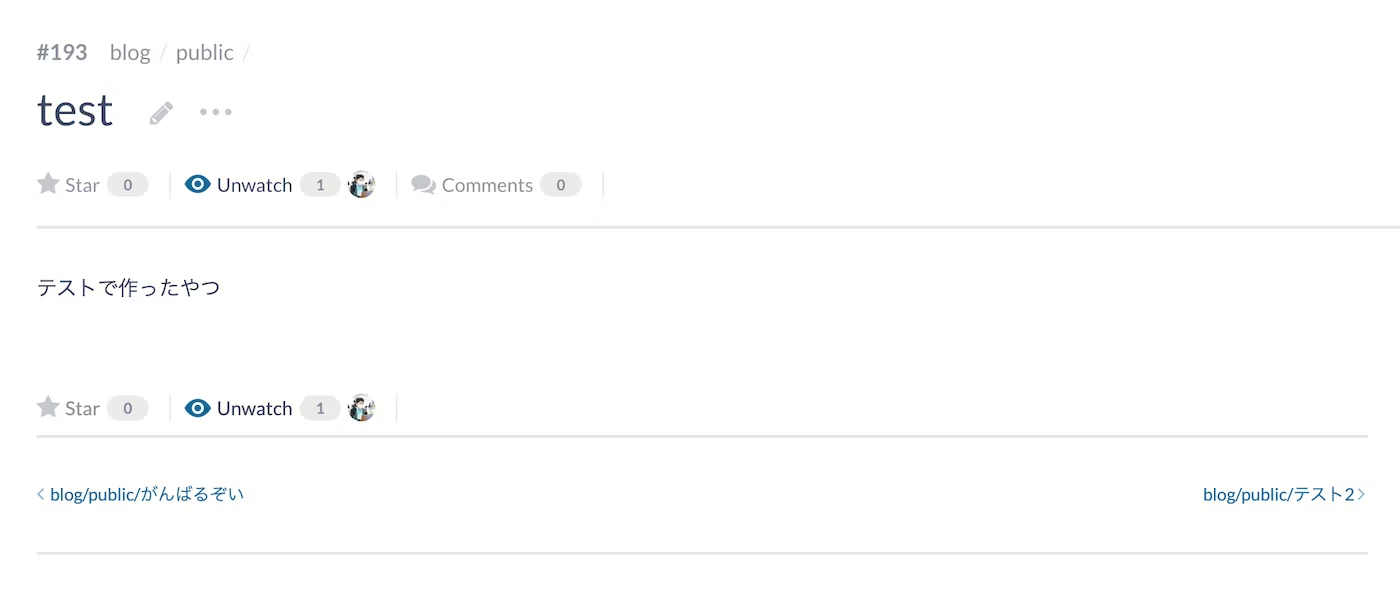
\includegraphics[width=8cm]{./image/02-chap9/esa-post-2.png}
    \caption{esaに投稿した記事2}
    \label{chap9-esa-post-2-image}
  \end{figure}

\section{GitHubの状態}

  しばらくすると、esaのWebhooksが走って、mdを保存してくれます。

  \begin{figure}[H]
    \centering
    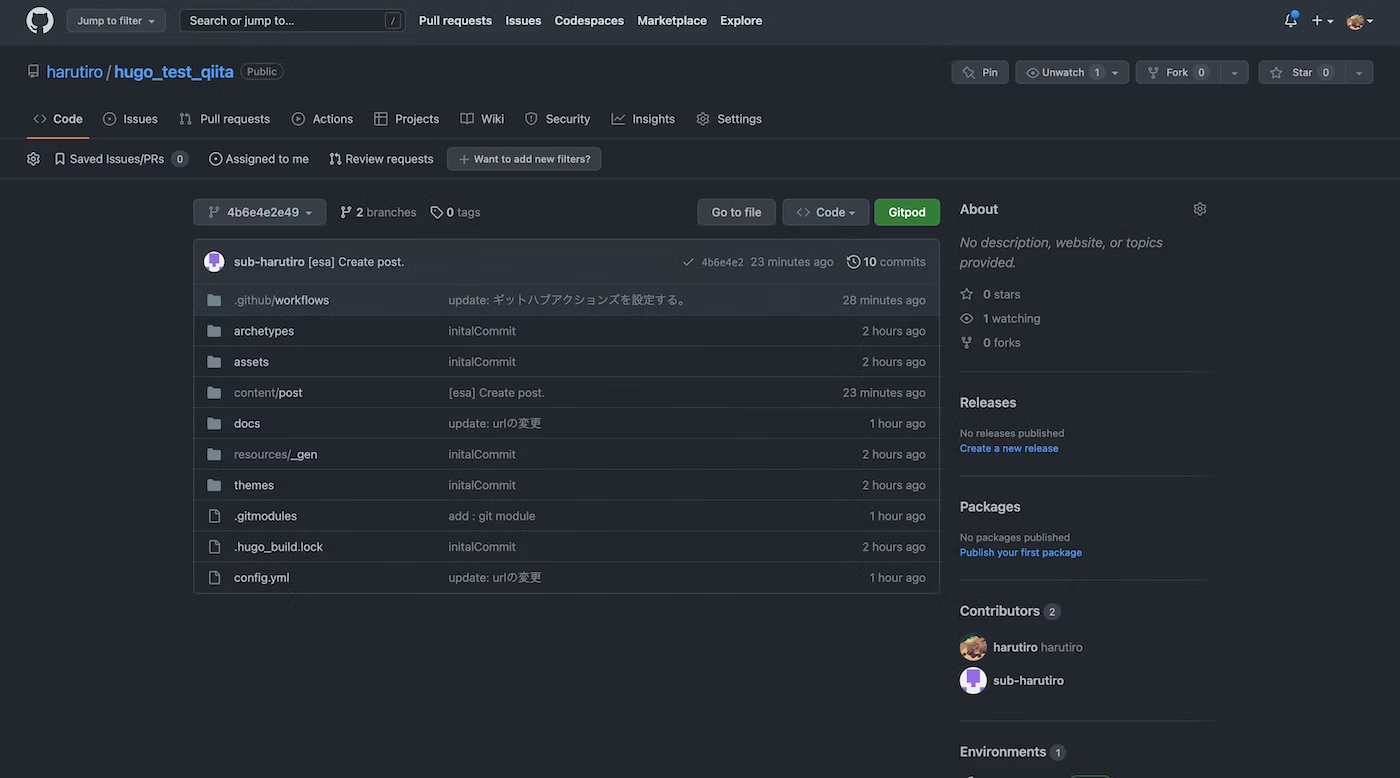
\includegraphics[width=8cm]{./image/02-chap9/git-repo.png}
    \caption{gitのリポジトリの状態}
    \label{chap9-git-repo-image}
  \end{figure}

\section{GitHub Actionsの状態}
  あたらしくPushされると、GitHub Actionsが走って、web$\_$publicのブランチに静的ファイルが生成されます。

  \begin{figure}[H]
    \centering
    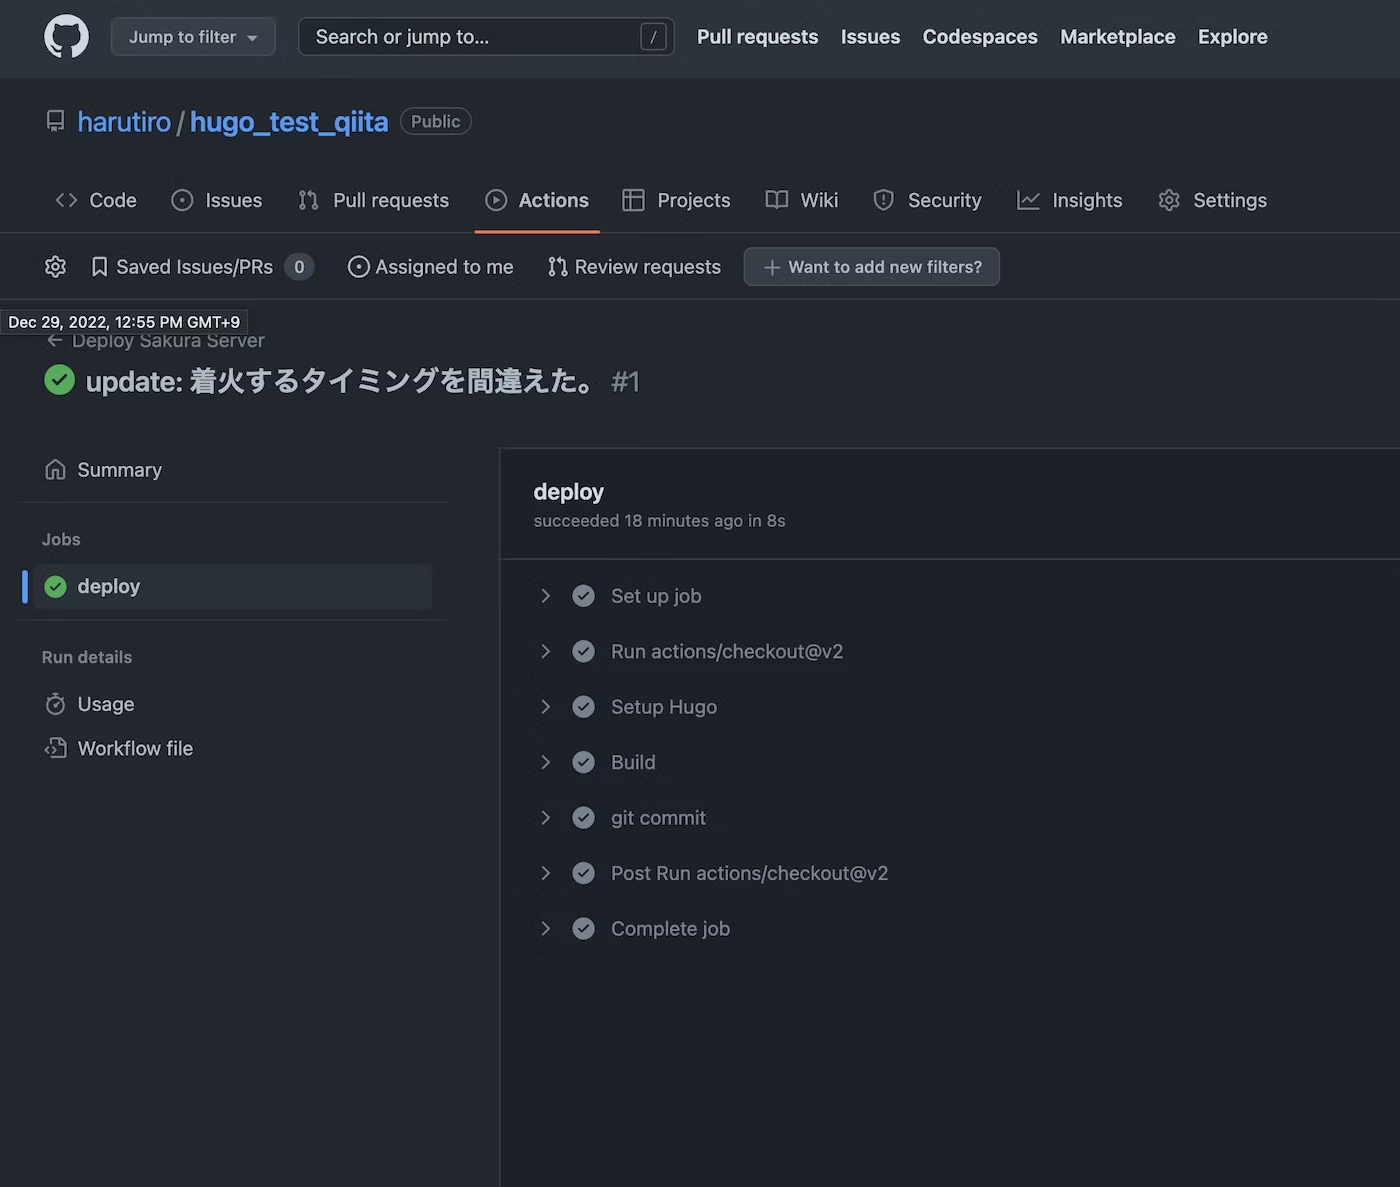
\includegraphics[width=8cm]{./image/02-chap9/git-action1.png}
    \caption{GitHub Actionsの状態}
    \label{chap9-git-action1-image}
  \end{figure}

  \begin{figure}[H]
    \centering
    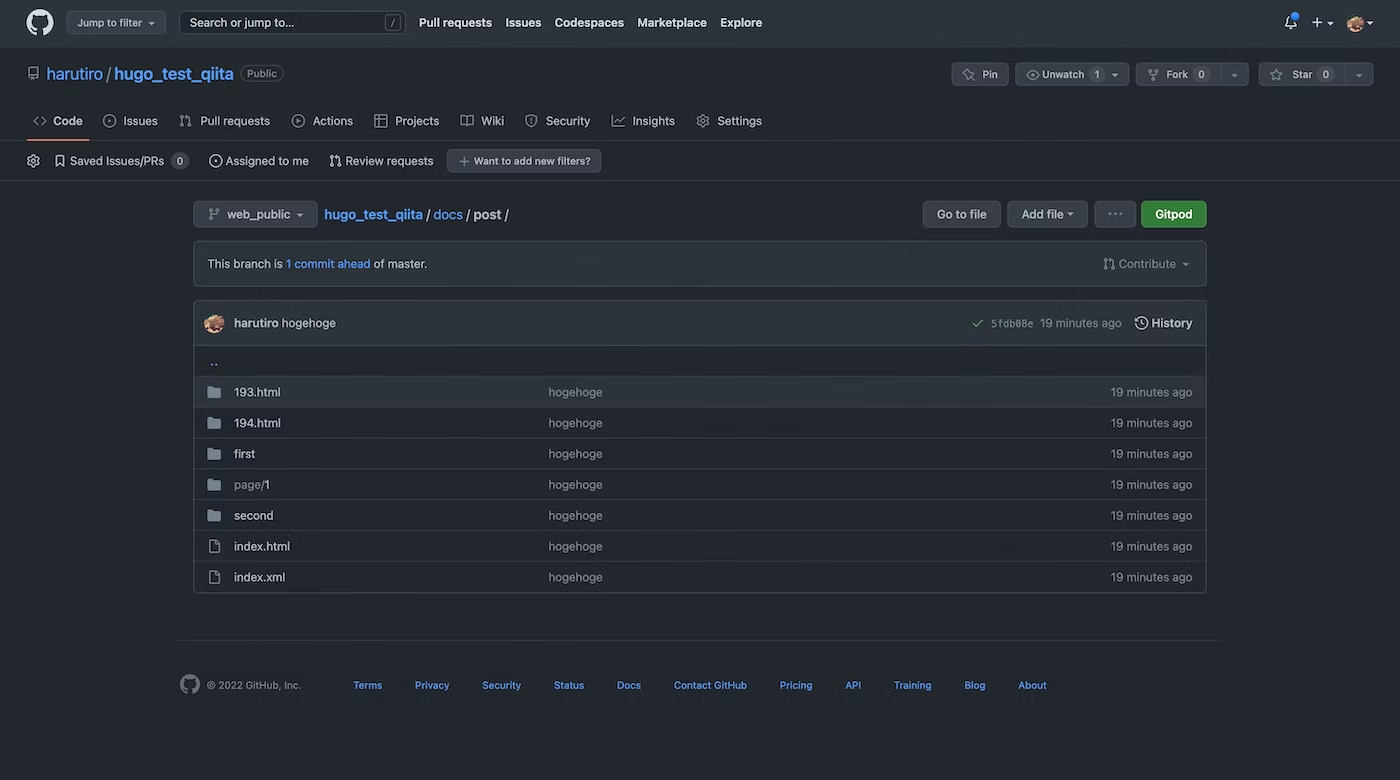
\includegraphics[width=8cm]{./image/02-chap9/git-action2.png}
    \caption{GitHub Actionsの状態 hugoの生成をしている状態}
    \label{chap9-git-action2-image}
  \end{figure}

\section{GitHub Pagesの状態}
  web$\_$publicにpushされるとGitHub Pagesが走って、自動的にデプロイされます。

  \begin{figure}[H]
    \centering
    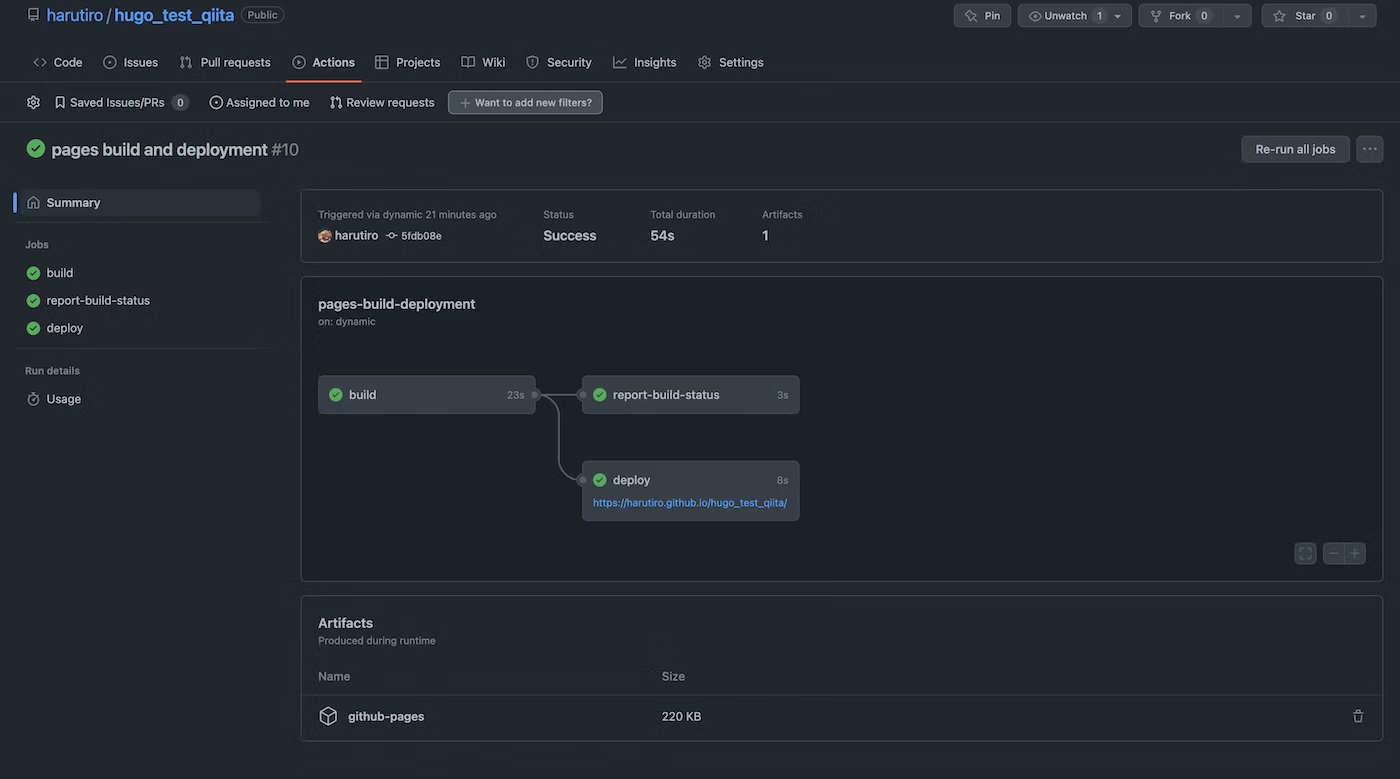
\includegraphics[width=8cm]{./image/02-chap9/git-pases.png}
    \caption{GitHub Pagesの状態}
    \label{chap9-git-pases-image}
  \end{figure}

\section{webページの状態}
  自動で更新がされていることが確認できました。

  \begin{figure}[H]
    \centering
    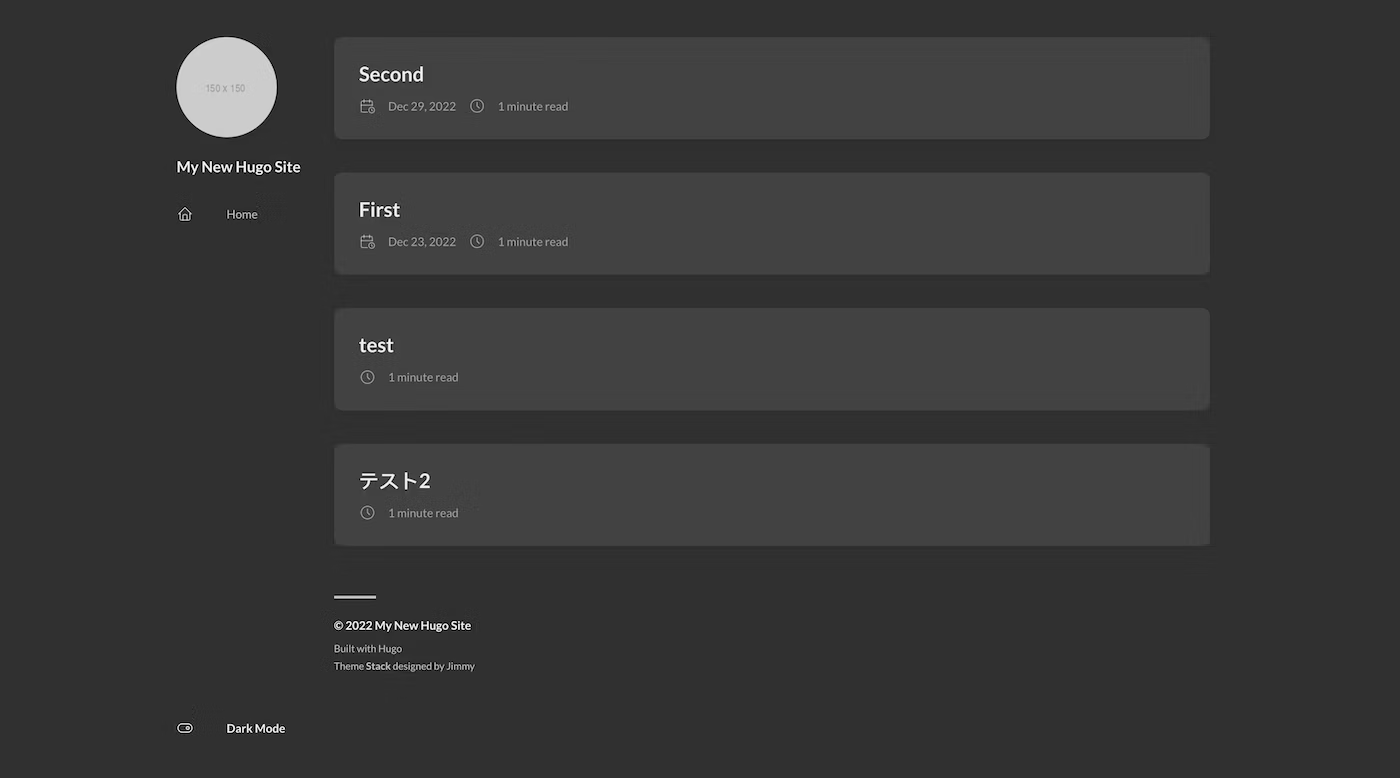
\includegraphics[width=8cm]{./image/02-chap9/hugo1.png}
    \caption{webページの状態}
    \label{chap9-hugo1-image}
  \end{figure}

  \begin{figure}[H]
    \centering
    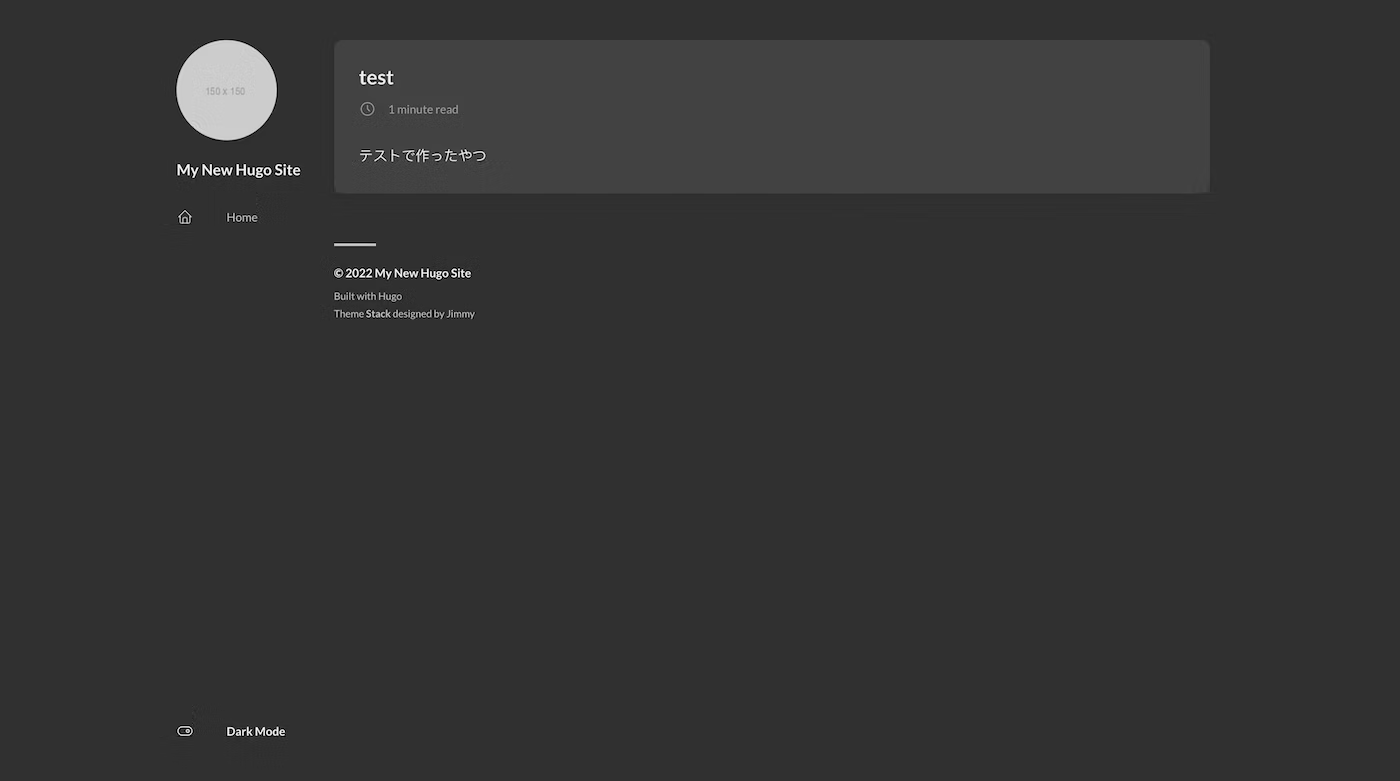
\includegraphics[width=8cm]{./image/02-chap9/hugo2.png}
    \caption{webページの状態 記事1}
    \label{chap9-hugo2-image}
  \end{figure}

  \begin{figure}[H]
    \centering
    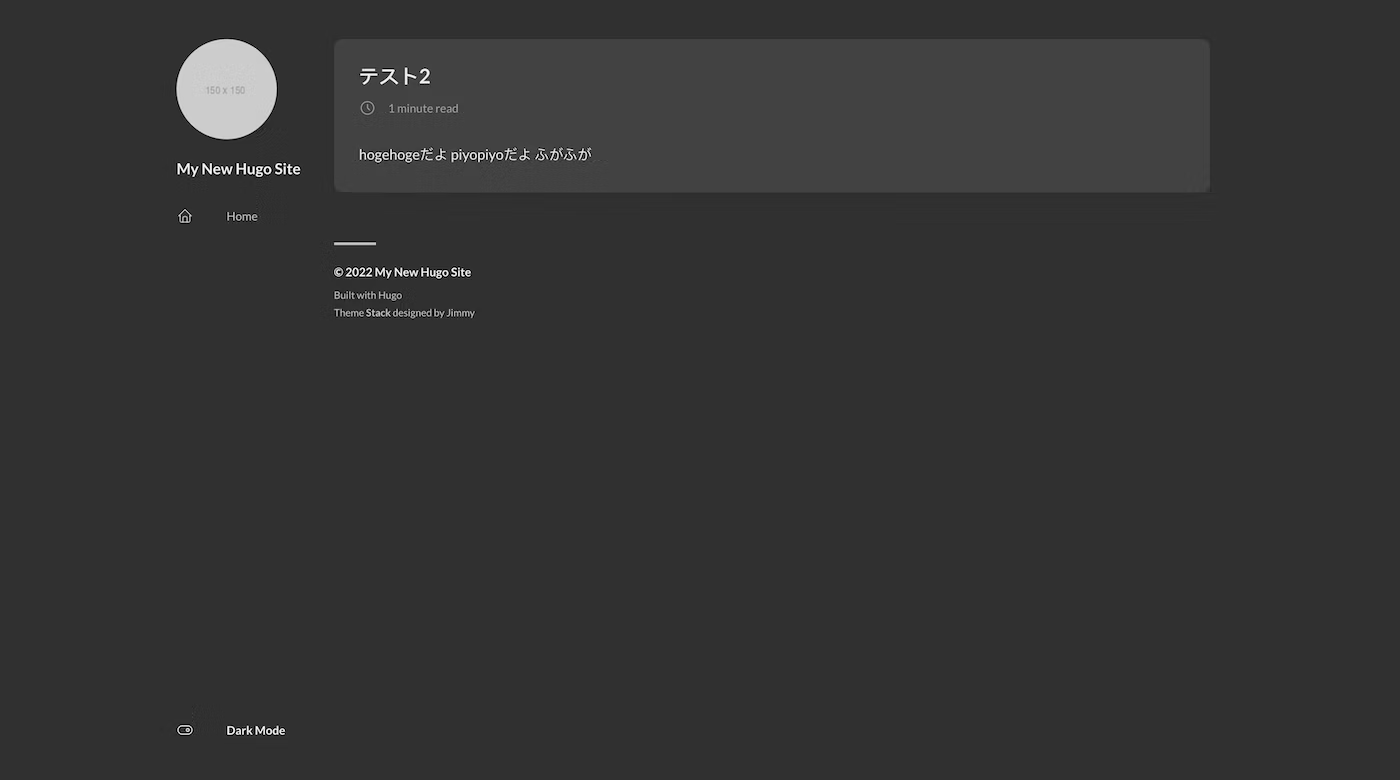
\includegraphics[width=8cm]{./image/02-chap9/hugo3.png}
    \caption{webページの状態 記事2}
    \label{chap9-hugo3-image}
  \end{figure}
\chapter{おわりに}

今回は、esaをCMSとして使い、GitHub Actionsで静的なWebサイトを作成して、GitHub Pagesで公開するということを行いました。

esaでは、設定からAPIを使うことで簡単にGitHubに記事を投稿することができます。
GitHub Actionsでは、GitHubにpushされたら自動でビルドを行い、GitHub Pagesに公開するということを行いました。
Hugoを使うことで、テンプレートを使って簡単に綺麗なWebサイトを作成することができます。

esa自体は、とてもいいサービスで、さまざまなAPIが公開されており、Slackと連携をしたり、GitHubと連携をしてバックアップを簡単にとることもできます。
複数人で一斉に編集をすることもできるため、私たちのサークルでは、情報共有のために使っています。

あまりesaをCMS化しようという試みがないかもしれませんが、大変便利なものなのでぜひ使ってみてはいかがでしょうか?
2022年/12月時点では、esaは学生団体でしたら、1年間無料で使えて更新も無料らしいので、ぜひ使ってみてください。


\bibliography{reference}
\bibliographystyle{junsrt}
\nocite{*}


\chapter{これはchapter}
\section{これはsection}
我輩は猫である\footnote{こんな感じで脚注を書く}。

どこで生れたかとんと見当がつかぬ。何でも薄暗いじめじめした所でニャーニャー泣いていた事だけは記憶している。吾輩はここで始めて人間というものを見た。しかもあとで聞くとそれは書生という人間中で一番獰悪な種族であったそうだ。この書生というのは時々我々を捕えて煮て食うという話である。

\begin{tcolorbox}[breakable]
\begin{verbatim}
1  /* ここにはソースコードを書く */
2  #include<stdio.h>
3
4  int main(void)
5  {
6    printf("Hello, World!\n");
7    return 0;
8  }
9  /* breakableを付けるとこんな感じで改行にも対応できる */
\end{verbatim}
\end{tcolorbox}

\begin{shaded}
\begin{verbatim}
## ここにはコマンドを書く
$ echo "Hello, World!"
\end{verbatim}
\end{shaded}

図表はキャプションを付けたときに、先頭に「▲」や「▼」を付けるようにした。

\begin{table}[H]
  \centering
  \caption{表のサンプル}
  \begin{tabular}{|c|l|l|l|} \hline
    日本 & hoge & fuga & piyo \\ \hline
    アメリカ & foo & bar & baz \\ \hline
  \end{tabular}
  \label{table-sample0402}
\end{table}

\begin{figure}[H]
  \centering
  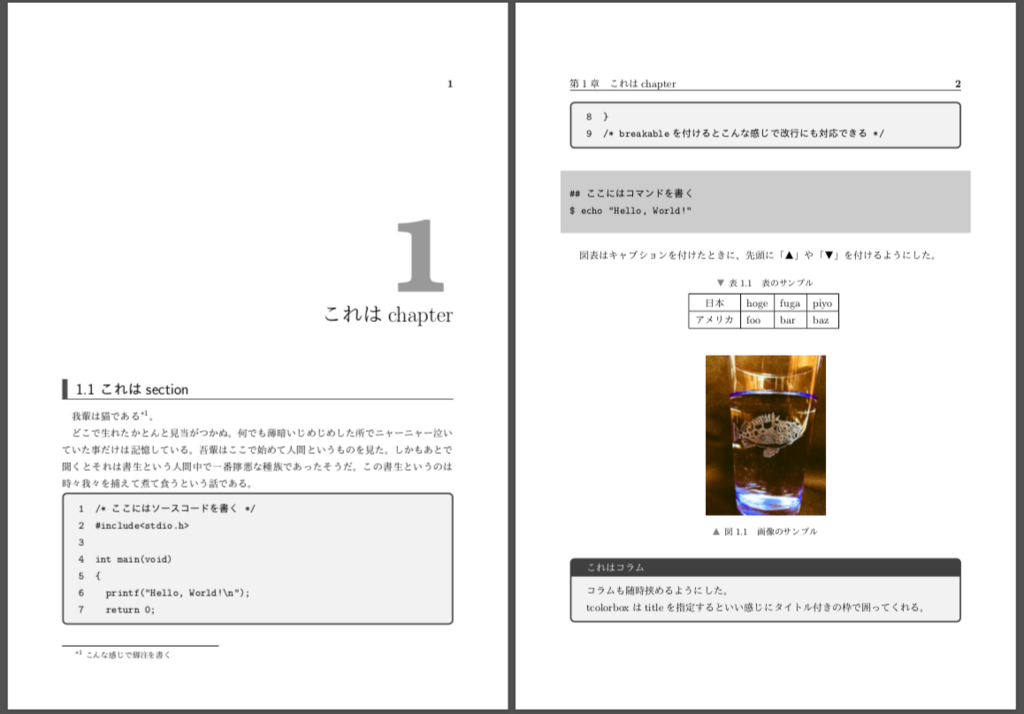
\includegraphics[width=4cm]{./image/sample.png}
  \caption{画像のサンプル}
  \label{figure-sample0402}
\end{figure}

\begin{tcolorbox}[title=これはコラム]
  コラムも随時挟めるようにした。

  tcolorboxはtitleを指定するといい感じにタイトル付きの枠で囲ってくれる。
\end{tcolorbox}






\end{document}